\documentclass[twoside]{book}

% Packages required by doxygen
\usepackage{fixltx2e}
\usepackage{calc}
\usepackage{doxygen}
\usepackage[export]{adjustbox} % also loads graphicx
\usepackage{graphicx}
\usepackage[utf8]{inputenc}
\usepackage{makeidx}
\usepackage{multicol}
\usepackage{multirow}
\PassOptionsToPackage{warn}{textcomp}
\usepackage{textcomp}
\usepackage[nointegrals]{wasysym}
\usepackage[table]{xcolor}

% Font selection
\usepackage[T1]{fontenc}
\usepackage[scaled=.90]{helvet}
\usepackage{courier}
\usepackage{amssymb}
\usepackage{sectsty}
\renewcommand{\familydefault}{\sfdefault}
\allsectionsfont{%
  \fontseries{bc}\selectfont%
  \color{darkgray}%
}
\renewcommand{\DoxyLabelFont}{%
  \fontseries{bc}\selectfont%
  \color{darkgray}%
}
\newcommand{\+}{\discretionary{\mbox{\scriptsize$\hookleftarrow$}}{}{}}

% Page & text layout
\usepackage{geometry}
\geometry{%
  a4paper,%
  top=2.5cm,%
  bottom=2.5cm,%
  left=2.5cm,%
  right=2.5cm%
}
\tolerance=750
\hfuzz=15pt
\hbadness=750
\setlength{\emergencystretch}{15pt}
\setlength{\parindent}{0cm}
\setlength{\parskip}{3ex plus 2ex minus 2ex}
\makeatletter
\renewcommand{\paragraph}{%
  \@startsection{paragraph}{4}{0ex}{-1.0ex}{1.0ex}{%
    \normalfont\normalsize\bfseries\SS@parafont%
  }%
}
\renewcommand{\subparagraph}{%
  \@startsection{subparagraph}{5}{0ex}{-1.0ex}{1.0ex}{%
    \normalfont\normalsize\bfseries\SS@subparafont%
  }%
}
\makeatother

% Headers & footers
\usepackage{fancyhdr}
\pagestyle{fancyplain}
\fancyhead[LE]{\fancyplain{}{\bfseries\thepage}}
\fancyhead[CE]{\fancyplain{}{}}
\fancyhead[RE]{\fancyplain{}{\bfseries\leftmark}}
\fancyhead[LO]{\fancyplain{}{\bfseries\rightmark}}
\fancyhead[CO]{\fancyplain{}{}}
\fancyhead[RO]{\fancyplain{}{\bfseries\thepage}}
\fancyfoot[LE]{\fancyplain{}{}}
\fancyfoot[CE]{\fancyplain{}{}}
\fancyfoot[RE]{\fancyplain{}{\bfseries\scriptsize Generated by Doxygen }}
\fancyfoot[LO]{\fancyplain{}{\bfseries\scriptsize Generated by Doxygen }}
\fancyfoot[CO]{\fancyplain{}{}}
\fancyfoot[RO]{\fancyplain{}{}}
\renewcommand{\footrulewidth}{0.4pt}
\renewcommand{\chaptermark}[1]{%
  \markboth{#1}{}%
}
\renewcommand{\sectionmark}[1]{%
  \markright{\thesection\ #1}%
}

% Indices & bibliography
\usepackage{natbib}
\usepackage[titles]{tocloft}
\setcounter{tocdepth}{3}
\setcounter{secnumdepth}{5}
\makeindex

% Hyperlinks (required, but should be loaded last)
\usepackage{ifpdf}
\ifpdf
  \usepackage[pdftex,pagebackref=true]{hyperref}
\else
  \usepackage[ps2pdf,pagebackref=true]{hyperref}
\fi
\hypersetup{%
  colorlinks=true,%
  linkcolor=blue,%
  citecolor=blue,%
  unicode%
}

% Custom commands
\newcommand{\clearemptydoublepage}{%
  \newpage{\pagestyle{empty}\cleardoublepage}%
}

\usepackage{caption}
\captionsetup{labelsep=space,justification=centering,font={bf},singlelinecheck=off,skip=4pt,position=top}

%===== C O N T E N T S =====

\begin{document}

% Titlepage & ToC
\hypersetup{pageanchor=false,
             bookmarksnumbered=true,
             pdfencoding=unicode
            }
\pagenumbering{alph}
\begin{titlepage}
\vspace*{7cm}
\begin{center}%
{\Large Turtlebot\+\_\+\+Navigation }\\
\vspace*{1cm}
{\large Generated by Doxygen 1.8.13}\\
\end{center}
\end{titlepage}
\clearemptydoublepage
\pagenumbering{roman}
\tableofcontents
\clearemptydoublepage
\pagenumbering{arabic}
\hypersetup{pageanchor=true}

%--- Begin generated contents ---
\chapter{Class Index}
\section{Class List}
Here are the classes, structs, unions and interfaces with brief descriptions\+:\begin{DoxyCompactList}
\item\contentsline{section}{\hyperlink{classrigid2d_1_1DiffDrive}{rigid2d\+::\+Diff\+Drive} \\*Implements high level abstraction and tracking of a diff drive robot }{\pageref{classrigid2d_1_1DiffDrive}}{}
\item\contentsline{section}{\hyperlink{classodometer}{odometer} \\*Implements methods for storing and updating a robot\textquotesingle{}s odometry data from published encoder data }{\pageref{classodometer}}{}
\item\contentsline{section}{\hyperlink{classrigid2d_1_1Transform2D}{rigid2d\+::\+Transform2D} \\*Rigid body transformation in 2 dimensions }{\pageref{classrigid2d_1_1Transform2D}}{}
\item\contentsline{section}{\hyperlink{classrigid2d_1_1Twist2D}{rigid2d\+::\+Twist2D} }{\pageref{classrigid2d_1_1Twist2D}}{}
\item\contentsline{section}{\hyperlink{structrigid2d_1_1Vector2D}{rigid2d\+::\+Vector2D} \\*A 2-\/\+Dimensional Vector }{\pageref{structrigid2d_1_1Vector2D}}{}
\item\contentsline{section}{\hyperlink{classrigid2d_1_1WayPoints}{rigid2d\+::\+Way\+Points} \\*Implements methods for navigating to a series of waypoints via a rotate and then translate strategy }{\pageref{classrigid2d_1_1WayPoints}}{}
\item\contentsline{section}{\hyperlink{structrigid2d_1_1WheelVelocities}{rigid2d\+::\+Wheel\+Velocities} \\*Desribes desired wheel velocities in radians/s }{\pageref{structrigid2d_1_1WheelVelocities}}{}
\end{DoxyCompactList}

\chapter{File Index}
\section{File List}
Here is a list of all documented files with brief descriptions\+:\begin{DoxyCompactList}
\item\contentsline{section}{src/rigid2d/include/rigid2d/\hyperlink{diff__drive_8hpp}{diff\+\_\+drive.\+hpp} \\*Implements high level abstraction and tracking of a diff drive robot }{\pageref{diff__drive_8hpp}}{}
\item\contentsline{section}{src/rigid2d/include/rigid2d/\hyperlink{rigid2d_8hpp}{rigid2d.\+hpp} \\*Library for two-\/dimensional rigid body transformations }{\pageref{rigid2d_8hpp}}{}
\item\contentsline{section}{src/rigid2d/include/rigid2d/\hyperlink{waypoints_8hpp}{waypoints.\+hpp} \\*Implements methods for navigating to a series of waypoints }{\pageref{waypoints_8hpp}}{}
\end{DoxyCompactList}

\chapter{Class Documentation}
\hypertarget{classrigid2d_1_1DiffDrive}{}\section{rigid2d\+:\+:Diff\+Drive Class Reference}
\label{classrigid2d_1_1DiffDrive}\index{rigid2d\+::\+Diff\+Drive@{rigid2d\+::\+Diff\+Drive}}


Implements high level abstraction and tracking of a diff drive robot.  




{\ttfamily \#include $<$diff\+\_\+drive.\+hpp$>$}



Collaboration diagram for rigid2d\+:\+:Diff\+Drive\+:
\nopagebreak
\begin{figure}[H]
\begin{center}
\leavevmode
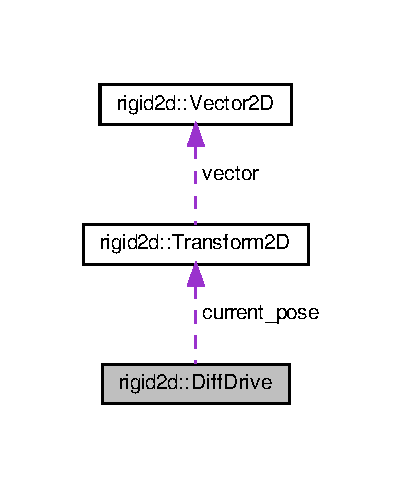
\includegraphics[width=194pt]{classrigid2d_1_1DiffDrive__coll__graph}
\end{center}
\end{figure}
\subsection*{Public Member Functions}
\begin{DoxyCompactItemize}
\item 
\mbox{\Hypertarget{classrigid2d_1_1DiffDrive_a2d646290b7a03d391a59e8a296fea30d}\label{classrigid2d_1_1DiffDrive_a2d646290b7a03d391a59e8a296fea30d}} 
\hyperlink{classrigid2d_1_1DiffDrive_a2d646290b7a03d391a59e8a296fea30d}{Diff\+Drive} ()
\begin{DoxyCompactList}\small\item\em The default constructor creates a robot at (0,0,0), with a fixed wheel base and wheel radius. \end{DoxyCompactList}\item 
\hyperlink{classrigid2d_1_1DiffDrive_a40b4756591df4548335371fea7bf60b4}{Diff\+Drive} (\hyperlink{classrigid2d_1_1Transform2D}{Transform2D}, double wheel\+\_\+base, double wheel\+\_\+radius)
\begin{DoxyCompactList}\small\item\em Constructor -\/ create a \hyperlink{classrigid2d_1_1DiffDrive}{Diff\+Drive} model by specifying the pose, and geometry. \end{DoxyCompactList}\item 
std\+::tuple$<$ double, double $>$ \hyperlink{classrigid2d_1_1DiffDrive_a9f8e57efccb3ea515c844e25828a373e}{get\+Encoders} (void)
\begin{DoxyCompactList}\small\item\em Compute the robot\textquotesingle{}s encoder values. \end{DoxyCompactList}\item 
\hyperlink{structrigid2d_1_1WheelVelocities}{Wheel\+Velocities} \hyperlink{classrigid2d_1_1DiffDrive_a62e097a7ce1162a9731f184679002573}{twist\+To\+Wheels} (\hyperlink{classrigid2d_1_1Twist2D}{Twist2D})
\begin{DoxyCompactList}\small\item\em Determine the wheel velocities required to make the robot move with the desired linear and angular velocities. \end{DoxyCompactList}\item 
\hyperlink{classrigid2d_1_1Twist2D}{Twist2D} \hyperlink{classrigid2d_1_1DiffDrive_a726f6bc97c6431bd80164e0403f36c2b}{wheels\+To\+Twist} (\hyperlink{structrigid2d_1_1WheelVelocities}{Wheel\+Velocities} vel)
\begin{DoxyCompactList}\small\item\em determine the body twist of the robot from its wheel velocities \end{DoxyCompactList}\item 
\hyperlink{structrigid2d_1_1WheelVelocities}{Wheel\+Velocities} \hyperlink{classrigid2d_1_1DiffDrive_af0ec14baf8f1bd40e1d55226f087ef74}{update\+Odometry} (double, double)
\begin{DoxyCompactList}\small\item\em Update the robot\textquotesingle{}s odometry based on the current encoder readings. \end{DoxyCompactList}\item 
void \hyperlink{classrigid2d_1_1DiffDrive_a87ba3d5ad02cef8285789a2cebe22961}{feedforward} (\hyperlink{classrigid2d_1_1Twist2D}{Twist2D})
\begin{DoxyCompactList}\small\item\em update the odometry of the diff drive robot, assuming that it follows the given body twist for one time unit \end{DoxyCompactList}\item 
geometry\+\_\+msgs\+::\+Pose2D \hyperlink{classrigid2d_1_1DiffDrive_ae4d0c4e53e8558fed8c7711724f585d3}{pose} ()
\begin{DoxyCompactList}\small\item\em Get the current pose of the robot. \end{DoxyCompactList}\item 
void \hyperlink{classrigid2d_1_1DiffDrive_a2554a9bce4ecada65a159498a432d444}{reset} (\hyperlink{classrigid2d_1_1Twist2D}{Twist2D} ps)
\begin{DoxyCompactList}\small\item\em reset the robot to the given position/orientation \end{DoxyCompactList}\item 
void \hyperlink{classrigid2d_1_1DiffDrive_a82198f5be806b6f772a1718f3887f5c9}{set\+Pose} (double x, double y, double theta)
\begin{DoxyCompactList}\small\item\em Set the robot\textquotesingle{}s pose. \end{DoxyCompactList}\item 
\mbox{\Hypertarget{classrigid2d_1_1DiffDrive_ac9e0ed189932445e27c86839b918b282}\label{classrigid2d_1_1DiffDrive_ac9e0ed189932445e27c86839b918b282}} 
\hyperlink{classrigid2d_1_1Transform2D}{Transform2D} {\bfseries get\+Pose} (void)
\end{DoxyCompactItemize}
\subsection*{Public Attributes}
\begin{DoxyCompactItemize}
\item 
\mbox{\Hypertarget{classrigid2d_1_1DiffDrive_a6d07f9fdff01d212a975386e7798f156}\label{classrigid2d_1_1DiffDrive_a6d07f9fdff01d212a975386e7798f156}} 
\hyperlink{classrigid2d_1_1Transform2D}{rigid2d\+::\+Transform2D} {\bfseries current\+\_\+pose}
\item 
\mbox{\Hypertarget{classrigid2d_1_1DiffDrive_ac98ca684c26df696998545c9061bdcef}\label{classrigid2d_1_1DiffDrive_ac98ca684c26df696998545c9061bdcef}} 
double {\bfseries wheel\+\_\+base}
\item 
\mbox{\Hypertarget{classrigid2d_1_1DiffDrive_aebc2a573e61f048b0e0817d38a56aa81}\label{classrigid2d_1_1DiffDrive_aebc2a573e61f048b0e0817d38a56aa81}} 
double {\bfseries wheel\+\_\+radius}
\item 
\mbox{\Hypertarget{classrigid2d_1_1DiffDrive_ae21880890a8cbcb1195a0e9e2b16fbe5}\label{classrigid2d_1_1DiffDrive_ae21880890a8cbcb1195a0e9e2b16fbe5}} 
double {\bfseries encoder\+\_\+left}
\item 
\mbox{\Hypertarget{classrigid2d_1_1DiffDrive_ac8d8b3b66fa054874f89f52dc25ac0bc}\label{classrigid2d_1_1DiffDrive_ac8d8b3b66fa054874f89f52dc25ac0bc}} 
double {\bfseries encoder\+\_\+right}
\end{DoxyCompactItemize}


\subsection{Detailed Description}
Implements high level abstraction and tracking of a diff drive robot. 

\subsection{Constructor \& Destructor Documentation}
\mbox{\Hypertarget{classrigid2d_1_1DiffDrive_a40b4756591df4548335371fea7bf60b4}\label{classrigid2d_1_1DiffDrive_a40b4756591df4548335371fea7bf60b4}} 
\index{rigid2d\+::\+Diff\+Drive@{rigid2d\+::\+Diff\+Drive}!Diff\+Drive@{Diff\+Drive}}
\index{Diff\+Drive@{Diff\+Drive}!rigid2d\+::\+Diff\+Drive@{rigid2d\+::\+Diff\+Drive}}
\subsubsection{\texorpdfstring{Diff\+Drive()}{DiffDrive()}}
{\footnotesize\ttfamily rigid2d\+::\+Diff\+Drive\+::\+Diff\+Drive (\begin{DoxyParamCaption}\item[{\hyperlink{classrigid2d_1_1Transform2D}{Transform2D}}]{,  }\item[{double}]{wheel\+\_\+base,  }\item[{double}]{wheel\+\_\+radius }\end{DoxyParamCaption})}



Constructor -\/ create a \hyperlink{classrigid2d_1_1DiffDrive}{Diff\+Drive} model by specifying the pose, and geometry. 


\begin{DoxyParams}{Parameters}
{\em pose} & -\/ the current position of the robot \\
\hline
{\em wheel\+\_\+base} & -\/ the distance between the wheel centers \\
\hline
{\em wheel\+\_\+radius} & -\/ the radius of the wheels \\
\hline
\end{DoxyParams}


\subsection{Member Function Documentation}
\mbox{\Hypertarget{classrigid2d_1_1DiffDrive_a87ba3d5ad02cef8285789a2cebe22961}\label{classrigid2d_1_1DiffDrive_a87ba3d5ad02cef8285789a2cebe22961}} 
\index{rigid2d\+::\+Diff\+Drive@{rigid2d\+::\+Diff\+Drive}!feedforward@{feedforward}}
\index{feedforward@{feedforward}!rigid2d\+::\+Diff\+Drive@{rigid2d\+::\+Diff\+Drive}}
\subsubsection{\texorpdfstring{feedforward()}{feedforward()}}
{\footnotesize\ttfamily void rigid2d\+::\+Diff\+Drive\+::feedforward (\begin{DoxyParamCaption}\item[{\hyperlink{classrigid2d_1_1Twist2D}{Twist2D}}]{ }\end{DoxyParamCaption})}



update the odometry of the diff drive robot, assuming that it follows the given body twist for one time unit 


\begin{DoxyParams}{Parameters}
{\em cmd} & -\/ the twist command to send to the robot \\
\hline
\end{DoxyParams}
\mbox{\Hypertarget{classrigid2d_1_1DiffDrive_a9f8e57efccb3ea515c844e25828a373e}\label{classrigid2d_1_1DiffDrive_a9f8e57efccb3ea515c844e25828a373e}} 
\index{rigid2d\+::\+Diff\+Drive@{rigid2d\+::\+Diff\+Drive}!get\+Encoders@{get\+Encoders}}
\index{get\+Encoders@{get\+Encoders}!rigid2d\+::\+Diff\+Drive@{rigid2d\+::\+Diff\+Drive}}
\subsubsection{\texorpdfstring{get\+Encoders()}{getEncoders()}}
{\footnotesize\ttfamily std\+::tuple$<$double, double$>$ rigid2d\+::\+Diff\+Drive\+::get\+Encoders (\begin{DoxyParamCaption}\item[{void}]{ }\end{DoxyParamCaption})}



Compute the robot\textquotesingle{}s encoder values. 

\begin{DoxyReturn}{Returns}
the robot\textquotesingle{}s current encoder values 
\end{DoxyReturn}
\mbox{\Hypertarget{classrigid2d_1_1DiffDrive_ae4d0c4e53e8558fed8c7711724f585d3}\label{classrigid2d_1_1DiffDrive_ae4d0c4e53e8558fed8c7711724f585d3}} 
\index{rigid2d\+::\+Diff\+Drive@{rigid2d\+::\+Diff\+Drive}!pose@{pose}}
\index{pose@{pose}!rigid2d\+::\+Diff\+Drive@{rigid2d\+::\+Diff\+Drive}}
\subsubsection{\texorpdfstring{pose()}{pose()}}
{\footnotesize\ttfamily geometry\+\_\+msgs\+::\+Pose2D rigid2d\+::\+Diff\+Drive\+::pose (\begin{DoxyParamCaption}{ }\end{DoxyParamCaption})}



Get the current pose of the robot. 

\begin{DoxyReturn}{Returns}
the current pose of the robot 
\end{DoxyReturn}
\mbox{\Hypertarget{classrigid2d_1_1DiffDrive_a2554a9bce4ecada65a159498a432d444}\label{classrigid2d_1_1DiffDrive_a2554a9bce4ecada65a159498a432d444}} 
\index{rigid2d\+::\+Diff\+Drive@{rigid2d\+::\+Diff\+Drive}!reset@{reset}}
\index{reset@{reset}!rigid2d\+::\+Diff\+Drive@{rigid2d\+::\+Diff\+Drive}}
\subsubsection{\texorpdfstring{reset()}{reset()}}
{\footnotesize\ttfamily void rigid2d\+::\+Diff\+Drive\+::reset (\begin{DoxyParamCaption}\item[{\hyperlink{classrigid2d_1_1Twist2D}{Twist2D}}]{ps }\end{DoxyParamCaption})}



reset the robot to the given position/orientation 


\begin{DoxyParams}{Parameters}
{\em ps} & -\/ the new pose of the robot \\
\hline
\end{DoxyParams}
\mbox{\Hypertarget{classrigid2d_1_1DiffDrive_a82198f5be806b6f772a1718f3887f5c9}\label{classrigid2d_1_1DiffDrive_a82198f5be806b6f772a1718f3887f5c9}} 
\index{rigid2d\+::\+Diff\+Drive@{rigid2d\+::\+Diff\+Drive}!set\+Pose@{set\+Pose}}
\index{set\+Pose@{set\+Pose}!rigid2d\+::\+Diff\+Drive@{rigid2d\+::\+Diff\+Drive}}
\subsubsection{\texorpdfstring{set\+Pose()}{setPose()}}
{\footnotesize\ttfamily void rigid2d\+::\+Diff\+Drive\+::set\+Pose (\begin{DoxyParamCaption}\item[{double}]{x,  }\item[{double}]{y,  }\item[{double}]{theta }\end{DoxyParamCaption})}



Set the robot\textquotesingle{}s pose. 


\begin{DoxyParams}{Parameters}
{\em x} & -\/ the new x coordinate \\
\hline
{\em y} & -\/ the new y coordinate \\
\hline
{\em theta} & -\/ the robot\textquotesingle{}s new angle in the plane \\
\hline
\end{DoxyParams}
\mbox{\Hypertarget{classrigid2d_1_1DiffDrive_a62e097a7ce1162a9731f184679002573}\label{classrigid2d_1_1DiffDrive_a62e097a7ce1162a9731f184679002573}} 
\index{rigid2d\+::\+Diff\+Drive@{rigid2d\+::\+Diff\+Drive}!twist\+To\+Wheels@{twist\+To\+Wheels}}
\index{twist\+To\+Wheels@{twist\+To\+Wheels}!rigid2d\+::\+Diff\+Drive@{rigid2d\+::\+Diff\+Drive}}
\subsubsection{\texorpdfstring{twist\+To\+Wheels()}{twistToWheels()}}
{\footnotesize\ttfamily \hyperlink{structrigid2d_1_1WheelVelocities}{Wheel\+Velocities} rigid2d\+::\+Diff\+Drive\+::twist\+To\+Wheels (\begin{DoxyParamCaption}\item[{\hyperlink{classrigid2d_1_1Twist2D}{Twist2D}}]{ }\end{DoxyParamCaption})}



Determine the wheel velocities required to make the robot move with the desired linear and angular velocities. 


\begin{DoxyParams}{Parameters}
{\em twist} & -\/ the desired twist in the body frame of the robot \\
\hline
\end{DoxyParams}
\begin{DoxyReturn}{Returns}
-\/ the wheel velocities to use 
\end{DoxyReturn}

\begin{DoxyExceptions}{Exceptions}
{\em std\+::exception} & \\
\hline
\end{DoxyExceptions}
\mbox{\Hypertarget{classrigid2d_1_1DiffDrive_af0ec14baf8f1bd40e1d55226f087ef74}\label{classrigid2d_1_1DiffDrive_af0ec14baf8f1bd40e1d55226f087ef74}} 
\index{rigid2d\+::\+Diff\+Drive@{rigid2d\+::\+Diff\+Drive}!update\+Odometry@{update\+Odometry}}
\index{update\+Odometry@{update\+Odometry}!rigid2d\+::\+Diff\+Drive@{rigid2d\+::\+Diff\+Drive}}
\subsubsection{\texorpdfstring{update\+Odometry()}{updateOdometry()}}
{\footnotesize\ttfamily \hyperlink{structrigid2d_1_1WheelVelocities}{Wheel\+Velocities} rigid2d\+::\+Diff\+Drive\+::update\+Odometry (\begin{DoxyParamCaption}\item[{double}]{,  }\item[{double}]{ }\end{DoxyParamCaption})}



Update the robot\textquotesingle{}s odometry based on the current encoder readings. 


\begin{DoxyParams}{Parameters}
{\em left} & -\/ the left encoder angle (in radians) \\
\hline
{\em right} & -\/ the right encoder angle (in radians) \\
\hline
\end{DoxyParams}
\mbox{\Hypertarget{classrigid2d_1_1DiffDrive_a726f6bc97c6431bd80164e0403f36c2b}\label{classrigid2d_1_1DiffDrive_a726f6bc97c6431bd80164e0403f36c2b}} 
\index{rigid2d\+::\+Diff\+Drive@{rigid2d\+::\+Diff\+Drive}!wheels\+To\+Twist@{wheels\+To\+Twist}}
\index{wheels\+To\+Twist@{wheels\+To\+Twist}!rigid2d\+::\+Diff\+Drive@{rigid2d\+::\+Diff\+Drive}}
\subsubsection{\texorpdfstring{wheels\+To\+Twist()}{wheelsToTwist()}}
{\footnotesize\ttfamily \hyperlink{classrigid2d_1_1Twist2D}{Twist2D} rigid2d\+::\+Diff\+Drive\+::wheels\+To\+Twist (\begin{DoxyParamCaption}\item[{\hyperlink{structrigid2d_1_1WheelVelocities}{Wheel\+Velocities}}]{vel }\end{DoxyParamCaption})}



determine the body twist of the robot from its wheel velocities 


\begin{DoxyParams}{Parameters}
{\em vel} & -\/ the velocities of the wheels, assumed to be held constant for one time unit \\
\hline
\end{DoxyParams}
\begin{DoxyReturn}{Returns}
the twist in the original body frame of the robot 
\end{DoxyReturn}


The documentation for this class was generated from the following file\+:\begin{DoxyCompactItemize}
\item 
src/rigid2d/include/rigid2d/\hyperlink{diff__drive_8hpp}{diff\+\_\+drive.\+hpp}\end{DoxyCompactItemize}

\hypertarget{classodometer}{}\section{odometer Class Reference}
\label{classodometer}\index{odometer@{odometer}}


Implements methods for storing and updating a robot\textquotesingle{}s odometry data from published encoder data.  




Collaboration diagram for odometer\+:
\nopagebreak
\begin{figure}[H]
\begin{center}
\leavevmode
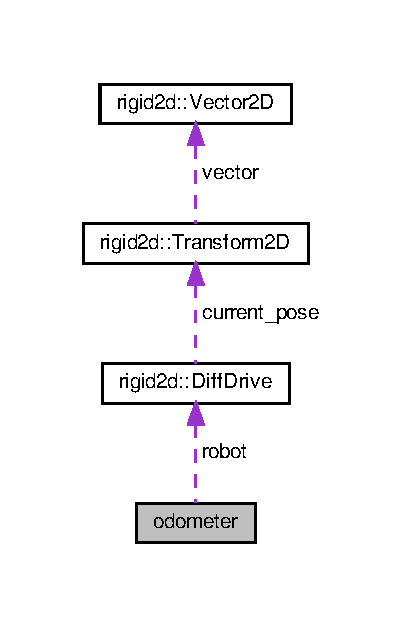
\includegraphics[width=194pt]{classodometer__coll__graph}
\end{center}
\end{figure}
\subsection*{Public Member Functions}
\begin{DoxyCompactItemize}
\item 
\mbox{\Hypertarget{classodometer_a72accc63053cf45e591d588e2c5c54b1}\label{classodometer_a72accc63053cf45e591d588e2c5c54b1}} 
bool \hyperlink{classodometer_a72accc63053cf45e591d588e2c5c54b1}{set\+\_\+pose\+\_\+srv} (rigid2d\+::set\+Pose\+::\+Request \&req, rigid2d\+::set\+Pose\+::\+Response \&res)
\begin{DoxyCompactList}\small\item\em Implements the set\+\_\+pose service Resets the robot to a new S\+E(2) configuration. \end{DoxyCompactList}\item 
std\+::tuple$<$ double, double $>$ \hyperlink{classodometer_a246018786026cc9d61b97c80f340e771}{get\+Wheel\+Positions} (sensor\+\_\+msgs\+::\+Joint\+State \&current\+\_\+joint\+\_\+state)
\begin{DoxyCompactList}\small\item\em Update the object\textquotesingle{}s fields tracking the robot\textquotesingle{}s wheel angles. \end{DoxyCompactList}\item 
void \hyperlink{classodometer_a70ae27127c495fde6b970b4ef432b326}{publish\+Marker} (const ros\+::\+Timer\+Event \&)
\item 
void \hyperlink{classodometer_a239d6c3386d056bd69978ae3021c4a55}{callback} (sensor\+\_\+msgs\+::\+Joint\+State current\+\_\+joint\+\_\+state)
\begin{DoxyCompactList}\small\item\em Functions runs when we recieve a new joint state message. \end{DoxyCompactList}\end{DoxyCompactItemize}
\subsection*{Public Attributes}
\begin{DoxyCompactItemize}
\item 
\mbox{\Hypertarget{classodometer_a773e2f50570c57bdcbf86a56b09a9630}\label{classodometer_a773e2f50570c57bdcbf86a56b09a9630}} 
ros\+::\+Node\+Handle {\bfseries n}
\item 
\mbox{\Hypertarget{classodometer_afcf3b6d28e203e698e5b42d213b337e9}\label{classodometer_afcf3b6d28e203e698e5b42d213b337e9}} 
std\+::string {\bfseries odom\+\_\+frame\+\_\+id}
\item 
\mbox{\Hypertarget{classodometer_a41f335bfc5071f6c8209fa9f35f56cf5}\label{classodometer_a41f335bfc5071f6c8209fa9f35f56cf5}} 
std\+::string {\bfseries body\+\_\+frame\+\_\+id}
\item 
\mbox{\Hypertarget{classodometer_a9dd1a055106627755635ed43a25b4586}\label{classodometer_a9dd1a055106627755635ed43a25b4586}} 
std\+::string {\bfseries left\+\_\+wheel\+\_\+joint}
\item 
\mbox{\Hypertarget{classodometer_a4c93f953fd318450895497f8e4554103}\label{classodometer_a4c93f953fd318450895497f8e4554103}} 
std\+::string {\bfseries right\+\_\+wheel\+\_\+joint}
\item 
\mbox{\Hypertarget{classodometer_a4a8b870a74d361ffe37f37edf054abb1}\label{classodometer_a4a8b870a74d361ffe37f37edf054abb1}} 
std\+::string {\bfseries base\+\_\+frame\+\_\+id}
\item 
\mbox{\Hypertarget{classodometer_ae9cdc488dd5c235b25aab107449bd1a5}\label{classodometer_ae9cdc488dd5c235b25aab107449bd1a5}} 
double {\bfseries wheel\+\_\+base}
\item 
\mbox{\Hypertarget{classodometer_a3956f99786cd6c01eadb97b83c2b9d9b}\label{classodometer_a3956f99786cd6c01eadb97b83c2b9d9b}} 
double {\bfseries wheel\+\_\+radius}
\item 
\mbox{\Hypertarget{classodometer_ab94a536e1b9a0e92d59acbfff618ac89}\label{classodometer_ab94a536e1b9a0e92d59acbfff618ac89}} 
double {\bfseries frequency}
\item 
\mbox{\Hypertarget{classodometer_a34f1a2ad42d8862ae1cc67ce106cf389}\label{classodometer_a34f1a2ad42d8862ae1cc67ce106cf389}} 
int {\bfseries marker\+Count}
\item 
\mbox{\Hypertarget{classodometer_a095f9edb9abe2c2f292e5601f16421bc}\label{classodometer_a095f9edb9abe2c2f292e5601f16421bc}} 
ros\+::\+Publisher {\bfseries marker\+\_\+pub}
\item 
\mbox{\Hypertarget{classodometer_ac8cb1419d75e761754625b8545f58db8}\label{classodometer_ac8cb1419d75e761754625b8545f58db8}} 
tf2\+\_\+ros\+::\+Transform\+Broadcaster {\bfseries odom\+\_\+broadcaster}
\item 
\mbox{\Hypertarget{classodometer_a1fbe3a51851f04f7e23d08ae9effce6e}\label{classodometer_a1fbe3a51851f04f7e23d08ae9effce6e}} 
ros\+::\+Publisher {\bfseries odom\+\_\+pub}
\item 
\mbox{\Hypertarget{classodometer_aaf5de7e9f79d6eec30f89e8fdf72768a}\label{classodometer_aaf5de7e9f79d6eec30f89e8fdf72768a}} 
ros\+::\+Subscriber {\bfseries sub}
\item 
\mbox{\Hypertarget{classodometer_abf9b513857c6af2fc2cbe26e17e3295a}\label{classodometer_abf9b513857c6af2fc2cbe26e17e3295a}} 
\hyperlink{classrigid2d_1_1DiffDrive}{rigid2d\+::\+Diff\+Drive} {\bfseries robot}
\item 
\mbox{\Hypertarget{classodometer_ad3e50ca62482e4768a49487b2c7938b8}\label{classodometer_ad3e50ca62482e4768a49487b2c7938b8}} 
ros\+::\+Timer {\bfseries timer}
\item 
\mbox{\Hypertarget{classodometer_a40093da249f61b22cf5fd3600135412e}\label{classodometer_a40093da249f61b22cf5fd3600135412e}} 
ros\+::\+Service\+Server {\bfseries set\+\_\+pose}
\end{DoxyCompactItemize}


\subsection{Detailed Description}
Implements methods for storing and updating a robot\textquotesingle{}s odometry data from published encoder data. 

Publishes\+: /odom, /visualization\+\_\+marker

Subscribes\+: /joint\+\_\+states

Services\+: /set\+\_\+pose -\/ Reset the robot to a new S\+E(2) configuration High level abstraction and trakcing of a robot\textquotesingle{}s odometry 

\subsection{Member Function Documentation}
\mbox{\Hypertarget{classodometer_a239d6c3386d056bd69978ae3021c4a55}\label{classodometer_a239d6c3386d056bd69978ae3021c4a55}} 
\index{odometer@{odometer}!callback@{callback}}
\index{callback@{callback}!odometer@{odometer}}
\subsubsection{\texorpdfstring{callback()}{callback()}}
{\footnotesize\ttfamily void odometer\+::callback (\begin{DoxyParamCaption}\item[{sensor\+\_\+msgs\+::\+Joint\+State}]{current\+\_\+joint\+\_\+state }\end{DoxyParamCaption})\hspace{0.3cm}{\ttfamily [inline]}}



Functions runs when we recieve a new joint state message. 


\begin{DoxyParams}{Parameters}
{\em current\+\_\+joint\+\_\+state} & -\/ The new state of the robot\textquotesingle{}s joints \\
\hline
\end{DoxyParams}
\mbox{\Hypertarget{classodometer_a246018786026cc9d61b97c80f340e771}\label{classodometer_a246018786026cc9d61b97c80f340e771}} 
\index{odometer@{odometer}!get\+Wheel\+Positions@{get\+Wheel\+Positions}}
\index{get\+Wheel\+Positions@{get\+Wheel\+Positions}!odometer@{odometer}}
\subsubsection{\texorpdfstring{get\+Wheel\+Positions()}{getWheelPositions()}}
{\footnotesize\ttfamily std\+::tuple$<$double, double$>$ odometer\+::get\+Wheel\+Positions (\begin{DoxyParamCaption}\item[{sensor\+\_\+msgs\+::\+Joint\+State \&}]{current\+\_\+joint\+\_\+state }\end{DoxyParamCaption})\hspace{0.3cm}{\ttfamily [inline]}}



Update the object\textquotesingle{}s fields tracking the robot\textquotesingle{}s wheel angles. 


\begin{DoxyParams}{Parameters}
{\em current\+\_\+joint\+\_\+state} & -\/ a message with the new wheel angles \\
\hline
\end{DoxyParams}
\mbox{\Hypertarget{classodometer_a70ae27127c495fde6b970b4ef432b326}\label{classodometer_a70ae27127c495fde6b970b4ef432b326}} 
\index{odometer@{odometer}!publish\+Marker@{publish\+Marker}}
\index{publish\+Marker@{publish\+Marker}!odometer@{odometer}}
\subsubsection{\texorpdfstring{publish\+Marker()}{publishMarker()}}
{\footnotesize\ttfamily void odometer\+::publish\+Marker (\begin{DoxyParamCaption}\item[{const ros\+::\+Timer\+Event \&}]{ }\end{DoxyParamCaption})\hspace{0.3cm}{\ttfamily [inline]}}

Publishes a marker for R\+V\+IZ of where the robot is 
\begin{DoxyParams}{Parameters}
{\em Timer\+Event} & is for R\+OS to use function with a R\+OS timer \\
\hline
\end{DoxyParams}


The documentation for this class was generated from the following file\+:\begin{DoxyCompactItemize}
\item 
src/rigid2d/src/odometer\+\_\+node.\+cpp\end{DoxyCompactItemize}

\hypertarget{classrigid2d_1_1Transform2D}{}\section{rigid2d\+:\+:Transform2D Class Reference}
\label{classrigid2d_1_1Transform2D}\index{rigid2d\+::\+Transform2D@{rigid2d\+::\+Transform2D}}


a rigid body transformation in 2 dimensions  




{\ttfamily \#include $<$rigid2d.\+hpp$>$}



Collaboration diagram for rigid2d\+:\+:Transform2D\+:
\nopagebreak
\begin{figure}[H]
\begin{center}
\leavevmode
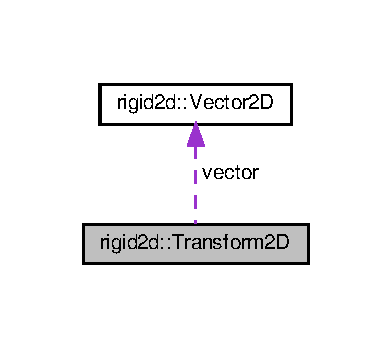
\includegraphics[width=188pt]{classrigid2d_1_1Transform2D__coll__graph}
\end{center}
\end{figure}
\subsection*{Public Member Functions}
\begin{DoxyCompactItemize}
\item 
\mbox{\Hypertarget{classrigid2d_1_1Transform2D_ac583ebfe4666feb4e42049ef0bf8ec3b}\label{classrigid2d_1_1Transform2D_ac583ebfe4666feb4e42049ef0bf8ec3b}} 
\hyperlink{classrigid2d_1_1Transform2D_ac583ebfe4666feb4e42049ef0bf8ec3b}{Transform2D} (void)
\begin{DoxyCompactList}\small\item\em Default Constructor. Creates the identity transformation. \end{DoxyCompactList}\item 
\hyperlink{classrigid2d_1_1Transform2D_ab3e595da2315ed50ba8eb24ead0c8d78}{Transform2D} (const \hyperlink{structrigid2d_1_1Vector2D}{Vector2D} \&trans)
\begin{DoxyCompactList}\small\item\em Create a transformation that is only a transformation without any rotation. \end{DoxyCompactList}\item 
\hyperlink{classrigid2d_1_1Transform2D_a3f2f654cb039320e331931c0877b39a3}{Transform2D} (double radians)
\item 
\hyperlink{classrigid2d_1_1Transform2D}{Transform2D} \hyperlink{classrigid2d_1_1Transform2D_a9d0ba77785a63d6299fe0671d8280584}{integrate\+Twist} (\hyperlink{classrigid2d_1_1Twist2D}{Twist2D})
\begin{DoxyCompactList}\small\item\em Integrate a constant twist for unit time So, if I am T\+\_\+sb and I apply the given twist for 1s then I end up at T\+\_\+bc. So, if I wanted T\+\_\+sc, then I would need to multiply T\+\_\+sb $\ast$ T\+\_\+sc. \end{DoxyCompactList}\item 
\hyperlink{classrigid2d_1_1Transform2D_a47de6c24f25c57da553a0fdaf13e2138}{Transform2D} (const \hyperlink{structrigid2d_1_1Vector2D}{Vector2D} \&trans, double radians)
\begin{DoxyCompactList}\small\item\em Create a transformation with a translational and rotational component. \end{DoxyCompactList}\item 
\hyperlink{classrigid2d_1_1Transform2D_a85302460b333608ad9e37cdbd71b78ac}{Transform2D} (const \hyperlink{structrigid2d_1_1Vector2D}{Vector2D} \&trans, double c\+Theta, double s\+Theta)
\begin{DoxyCompactList}\small\item\em Create a transformation which has both a rotation and a translation. \end{DoxyCompactList}\item 
geometry\+\_\+msgs\+::\+Pose \hyperlink{classrigid2d_1_1Transform2D_aedcb4e4472f57e774ddf21b441c7967f}{displacement} ()
\begin{DoxyCompactList}\small\item\em Compute the x, y, theta of the Transform as a Pose. \end{DoxyCompactList}\item 
\hyperlink{structrigid2d_1_1Vector2D}{Vector2D} \hyperlink{classrigid2d_1_1Transform2D_aab68d8df21419767d4291e226e0a3481}{operator()} (\hyperlink{structrigid2d_1_1Vector2D}{Vector2D} v) const
\begin{DoxyCompactList}\small\item\em Apply the transformation to the vector v. \end{DoxyCompactList}\item 
\hyperlink{classrigid2d_1_1Twist2D}{Twist2D} \hyperlink{classrigid2d_1_1Transform2D_a64346bd397406cf26e12d3022a3c3dee}{operator()} (\hyperlink{classrigid2d_1_1Twist2D}{Twist2D} twist)
\begin{DoxyCompactList}\small\item\em Uses adjoint to map a twist from one frame to another See page 85 of Modern Robotics for more details. Since this is planar motion, the adjoint simplifies down to a pretty nice little set of expressions. Initially, I constructed the whole 6x6 matrix but decided this was likely a better implementation. \end{DoxyCompactList}\item 
\hyperlink{classrigid2d_1_1Transform2D}{Transform2D} \hyperlink{classrigid2d_1_1Transform2D_a921bb5138fd83e48aaf75349dfd51653}{inv} () const
\begin{DoxyCompactList}\small\item\em Computes and returns the inverse of the given S\+E(2) matrix Instead of constructing the entire matrix in Eigen and inverting, I opt to use the properties of S\+E(2) matrices. This should help reduce the amount of numerical error See Modern Robotics chapter 3 for properties of S\+E(2) matrices. \end{DoxyCompactList}\item 
\hyperlink{classrigid2d_1_1Transform2D}{Transform2D} \& \hyperlink{classrigid2d_1_1Transform2D_ae832dd7b1488f6440ba2f98e95b684b5}{operator$\ast$=} (const \hyperlink{classrigid2d_1_1Transform2D}{Transform2D} \&rhs)
\begin{DoxyCompactList}\small\item\em Does comparsion of two Transform2\+Ds This is useful for testing to see if two transforms are equal. \end{DoxyCompactList}\item 
double \hyperlink{classrigid2d_1_1Transform2D_a2670394279fdfe595d859a1deab2b93f}{getX} (void) const
\begin{DoxyCompactList}\small\item\em Get and return x component of the twist. \end{DoxyCompactList}\item 
double \hyperlink{classrigid2d_1_1Transform2D_a8557f7ba90f5bc8ae468b56662e518e3}{getY} (void) const
\begin{DoxyCompactList}\small\item\em Get and return y component of the twist. \end{DoxyCompactList}\item 
double \hyperlink{classrigid2d_1_1Transform2D_aa380770351c67c0cd4410ceeb82b7c0d}{get\+Theta} (void) const
\begin{DoxyCompactList}\small\item\em Uses the stored cos(theta) and sin(theta) fields to recover theta. \end{DoxyCompactList}\item 
double \hyperlink{classrigid2d_1_1Transform2D_ae713c7af107cfd4ba9819f1a16e743d1}{get\+C\+Theta} (void) const
\begin{DoxyCompactList}\small\item\em Retrieves the cos of the current angle. \end{DoxyCompactList}\item 
double \hyperlink{classrigid2d_1_1Transform2D_a980917a1d86f290bd931dfa3eb78144f}{get\+S\+Theta} (void) const
\begin{DoxyCompactList}\small\item\em Retreives the sin of the current angle. \end{DoxyCompactList}\end{DoxyCompactItemize}
\subsection*{Public Attributes}
\begin{DoxyCompactItemize}
\item 
\mbox{\Hypertarget{classrigid2d_1_1Transform2D_a660fa2c66318224d29ac888e149e3f5d}\label{classrigid2d_1_1Transform2D_a660fa2c66318224d29ac888e149e3f5d}} 
\hyperlink{structrigid2d_1_1Vector2D}{Vector2D} {\bfseries vector}
\item 
\mbox{\Hypertarget{classrigid2d_1_1Transform2D_aecc32fb172617e9283d2fb6ab63093e0}\label{classrigid2d_1_1Transform2D_aecc32fb172617e9283d2fb6ab63093e0}} 
double {\bfseries s\+Theta}
\item 
\mbox{\Hypertarget{classrigid2d_1_1Transform2D_a2af0344e3d1b6e551317ff6784661ac5}\label{classrigid2d_1_1Transform2D_a2af0344e3d1b6e551317ff6784661ac5}} 
double {\bfseries c\+Theta}
\end{DoxyCompactItemize}
\subsection*{Friends}
\begin{DoxyCompactItemize}
\item 
std\+::ostream \& \hyperlink{classrigid2d_1_1Transform2D_ad5239a3fa3a0f9cebd73c39f34c2075f}{operator$<$$<$} (std\+::ostream \&os, const \hyperlink{classrigid2d_1_1Transform2D}{Transform2D} \&tf)
\begin{DoxyCompactList}\small\item\em Print a human readable description of the twist. \end{DoxyCompactList}\end{DoxyCompactItemize}


\subsection{Detailed Description}
a rigid body transformation in 2 dimensions 

\subsection{Constructor \& Destructor Documentation}
\mbox{\Hypertarget{classrigid2d_1_1Transform2D_ab3e595da2315ed50ba8eb24ead0c8d78}\label{classrigid2d_1_1Transform2D_ab3e595da2315ed50ba8eb24ead0c8d78}} 
\index{rigid2d\+::\+Transform2D@{rigid2d\+::\+Transform2D}!Transform2D@{Transform2D}}
\index{Transform2D@{Transform2D}!rigid2d\+::\+Transform2D@{rigid2d\+::\+Transform2D}}
\subsubsection{\texorpdfstring{Transform2\+D()}{Transform2D()}\hspace{0.1cm}{\footnotesize\ttfamily [1/4]}}
{\footnotesize\ttfamily rigid2d\+::\+Transform2\+D\+::\+Transform2D (\begin{DoxyParamCaption}\item[{const \hyperlink{structrigid2d_1_1Vector2D}{Vector2D} \&}]{trans }\end{DoxyParamCaption})\hspace{0.3cm}{\ttfamily [explicit]}}



Create a transformation that is only a transformation without any rotation. 


\begin{DoxyParams}{Parameters}
{\em p} & -\/ the vector describing the frame\textquotesingle{}s displacement \\
\hline
\end{DoxyParams}
\mbox{\Hypertarget{classrigid2d_1_1Transform2D_a3f2f654cb039320e331931c0877b39a3}\label{classrigid2d_1_1Transform2D_a3f2f654cb039320e331931c0877b39a3}} 
\index{rigid2d\+::\+Transform2D@{rigid2d\+::\+Transform2D}!Transform2D@{Transform2D}}
\index{Transform2D@{Transform2D}!rigid2d\+::\+Transform2D@{rigid2d\+::\+Transform2D}}
\subsubsection{\texorpdfstring{Transform2\+D()}{Transform2D()}\hspace{0.1cm}{\footnotesize\ttfamily [2/4]}}
{\footnotesize\ttfamily rigid2d\+::\+Transform2\+D\+::\+Transform2D (\begin{DoxyParamCaption}\item[{double}]{radians }\end{DoxyParamCaption})\hspace{0.3cm}{\ttfamily [explicit]}}

Constructor for \hyperlink{classrigid2d_1_1Transform2D}{Transform2D} which creates a twist which is just a rotation 
\begin{DoxyParams}{Parameters}
{\em radians} & -\/ the angle of rotation about the z-\/axis \\
\hline
\end{DoxyParams}
\mbox{\Hypertarget{classrigid2d_1_1Transform2D_a47de6c24f25c57da553a0fdaf13e2138}\label{classrigid2d_1_1Transform2D_a47de6c24f25c57da553a0fdaf13e2138}} 
\index{rigid2d\+::\+Transform2D@{rigid2d\+::\+Transform2D}!Transform2D@{Transform2D}}
\index{Transform2D@{Transform2D}!rigid2d\+::\+Transform2D@{rigid2d\+::\+Transform2D}}
\subsubsection{\texorpdfstring{Transform2\+D()}{Transform2D()}\hspace{0.1cm}{\footnotesize\ttfamily [3/4]}}
{\footnotesize\ttfamily rigid2d\+::\+Transform2\+D\+::\+Transform2D (\begin{DoxyParamCaption}\item[{const \hyperlink{structrigid2d_1_1Vector2D}{Vector2D} \&}]{trans,  }\item[{double}]{radians }\end{DoxyParamCaption})}



Create a transformation with a translational and rotational component. 


\begin{DoxyParams}{Parameters}
{\em trans} & -\/ the translation \\
\hline
{\em rot} & -\/ the rotation, in radians \\
\hline
\end{DoxyParams}
\mbox{\Hypertarget{classrigid2d_1_1Transform2D_a85302460b333608ad9e37cdbd71b78ac}\label{classrigid2d_1_1Transform2D_a85302460b333608ad9e37cdbd71b78ac}} 
\index{rigid2d\+::\+Transform2D@{rigid2d\+::\+Transform2D}!Transform2D@{Transform2D}}
\index{Transform2D@{Transform2D}!rigid2d\+::\+Transform2D@{rigid2d\+::\+Transform2D}}
\subsubsection{\texorpdfstring{Transform2\+D()}{Transform2D()}\hspace{0.1cm}{\footnotesize\ttfamily [4/4]}}
{\footnotesize\ttfamily rigid2d\+::\+Transform2\+D\+::\+Transform2D (\begin{DoxyParamCaption}\item[{const \hyperlink{structrigid2d_1_1Vector2D}{Vector2D} \&}]{trans,  }\item[{double}]{c\+Theta,  }\item[{double}]{s\+Theta }\end{DoxyParamCaption})}



Create a transformation which has both a rotation and a translation. 


\begin{DoxyParams}{Parameters}
{\em trans} & -\/ vector describing translation \\
\hline
{\em radians} & -\/ orientation about z-\/axis \\
\hline
\end{DoxyParams}


\subsection{Member Function Documentation}
\mbox{\Hypertarget{classrigid2d_1_1Transform2D_aedcb4e4472f57e774ddf21b441c7967f}\label{classrigid2d_1_1Transform2D_aedcb4e4472f57e774ddf21b441c7967f}} 
\index{rigid2d\+::\+Transform2D@{rigid2d\+::\+Transform2D}!displacement@{displacement}}
\index{displacement@{displacement}!rigid2d\+::\+Transform2D@{rigid2d\+::\+Transform2D}}
\subsubsection{\texorpdfstring{displacement()}{displacement()}}
{\footnotesize\ttfamily geometry\+\_\+msgs\+::\+Pose rigid2d\+::\+Transform2\+D\+::displacement (\begin{DoxyParamCaption}{ }\end{DoxyParamCaption})}



Compute the x, y, theta of the Transform as a Pose. 

\begin{DoxyReturn}{Returns}
the x, y, theta of the Transform as a Pose 
\end{DoxyReturn}
\mbox{\Hypertarget{classrigid2d_1_1Transform2D_ae713c7af107cfd4ba9819f1a16e743d1}\label{classrigid2d_1_1Transform2D_ae713c7af107cfd4ba9819f1a16e743d1}} 
\index{rigid2d\+::\+Transform2D@{rigid2d\+::\+Transform2D}!get\+C\+Theta@{get\+C\+Theta}}
\index{get\+C\+Theta@{get\+C\+Theta}!rigid2d\+::\+Transform2D@{rigid2d\+::\+Transform2D}}
\subsubsection{\texorpdfstring{get\+C\+Theta()}{getCTheta()}}
{\footnotesize\ttfamily double rigid2d\+::\+Transform2\+D\+::get\+C\+Theta (\begin{DoxyParamCaption}\item[{void}]{ }\end{DoxyParamCaption}) const}



Retrieves the cos of the current angle. 

\begin{DoxyReturn}{Returns}
the cos of the current angle in the plane 
\end{DoxyReturn}
\mbox{\Hypertarget{classrigid2d_1_1Transform2D_a980917a1d86f290bd931dfa3eb78144f}\label{classrigid2d_1_1Transform2D_a980917a1d86f290bd931dfa3eb78144f}} 
\index{rigid2d\+::\+Transform2D@{rigid2d\+::\+Transform2D}!get\+S\+Theta@{get\+S\+Theta}}
\index{get\+S\+Theta@{get\+S\+Theta}!rigid2d\+::\+Transform2D@{rigid2d\+::\+Transform2D}}
\subsubsection{\texorpdfstring{get\+S\+Theta()}{getSTheta()}}
{\footnotesize\ttfamily double rigid2d\+::\+Transform2\+D\+::get\+S\+Theta (\begin{DoxyParamCaption}\item[{void}]{ }\end{DoxyParamCaption}) const}



Retreives the sin of the current angle. 

\begin{DoxyReturn}{Returns}
the sin of the current angle in the plane 
\end{DoxyReturn}
\mbox{\Hypertarget{classrigid2d_1_1Transform2D_aa380770351c67c0cd4410ceeb82b7c0d}\label{classrigid2d_1_1Transform2D_aa380770351c67c0cd4410ceeb82b7c0d}} 
\index{rigid2d\+::\+Transform2D@{rigid2d\+::\+Transform2D}!get\+Theta@{get\+Theta}}
\index{get\+Theta@{get\+Theta}!rigid2d\+::\+Transform2D@{rigid2d\+::\+Transform2D}}
\subsubsection{\texorpdfstring{get\+Theta()}{getTheta()}}
{\footnotesize\ttfamily double rigid2d\+::\+Transform2\+D\+::get\+Theta (\begin{DoxyParamCaption}\item[{void}]{ }\end{DoxyParamCaption}) const}



Uses the stored cos(theta) and sin(theta) fields to recover theta. 

\begin{DoxyReturn}{Returns}
theta in radians 
\end{DoxyReturn}
\mbox{\Hypertarget{classrigid2d_1_1Transform2D_a2670394279fdfe595d859a1deab2b93f}\label{classrigid2d_1_1Transform2D_a2670394279fdfe595d859a1deab2b93f}} 
\index{rigid2d\+::\+Transform2D@{rigid2d\+::\+Transform2D}!getX@{getX}}
\index{getX@{getX}!rigid2d\+::\+Transform2D@{rigid2d\+::\+Transform2D}}
\subsubsection{\texorpdfstring{get\+X()}{getX()}}
{\footnotesize\ttfamily double rigid2d\+::\+Transform2\+D\+::getX (\begin{DoxyParamCaption}\item[{void}]{ }\end{DoxyParamCaption}) const}



Get and return x component of the twist. 

\begin{DoxyReturn}{Returns}
the x component of the twist 
\end{DoxyReturn}
\mbox{\Hypertarget{classrigid2d_1_1Transform2D_a8557f7ba90f5bc8ae468b56662e518e3}\label{classrigid2d_1_1Transform2D_a8557f7ba90f5bc8ae468b56662e518e3}} 
\index{rigid2d\+::\+Transform2D@{rigid2d\+::\+Transform2D}!getY@{getY}}
\index{getY@{getY}!rigid2d\+::\+Transform2D@{rigid2d\+::\+Transform2D}}
\subsubsection{\texorpdfstring{get\+Y()}{getY()}}
{\footnotesize\ttfamily double rigid2d\+::\+Transform2\+D\+::getY (\begin{DoxyParamCaption}\item[{void}]{ }\end{DoxyParamCaption}) const}



Get and return y component of the twist. 

\begin{DoxyReturn}{Returns}
the y component of the twist 
\end{DoxyReturn}
\mbox{\Hypertarget{classrigid2d_1_1Transform2D_a9d0ba77785a63d6299fe0671d8280584}\label{classrigid2d_1_1Transform2D_a9d0ba77785a63d6299fe0671d8280584}} 
\index{rigid2d\+::\+Transform2D@{rigid2d\+::\+Transform2D}!integrate\+Twist@{integrate\+Twist}}
\index{integrate\+Twist@{integrate\+Twist}!rigid2d\+::\+Transform2D@{rigid2d\+::\+Transform2D}}
\subsubsection{\texorpdfstring{integrate\+Twist()}{integrateTwist()}}
{\footnotesize\ttfamily \hyperlink{classrigid2d_1_1Transform2D}{Transform2D} rigid2d\+::\+Transform2\+D\+::integrate\+Twist (\begin{DoxyParamCaption}\item[{\hyperlink{classrigid2d_1_1Twist2D}{Twist2D}}]{ }\end{DoxyParamCaption})}



Integrate a constant twist for unit time So, if I am T\+\_\+sb and I apply the given twist for 1s then I end up at T\+\_\+bc. So, if I wanted T\+\_\+sc, then I would need to multiply T\+\_\+sb $\ast$ T\+\_\+sc. 


\begin{DoxyParams}{Parameters}
{\em t} & -\/ the twist \\
\hline
\end{DoxyParams}
\begin{DoxyReturn}{Returns}
the new frame relative to the old/prior one Important -\/ this function assumes unit time! 
\end{DoxyReturn}
\mbox{\Hypertarget{classrigid2d_1_1Transform2D_a921bb5138fd83e48aaf75349dfd51653}\label{classrigid2d_1_1Transform2D_a921bb5138fd83e48aaf75349dfd51653}} 
\index{rigid2d\+::\+Transform2D@{rigid2d\+::\+Transform2D}!inv@{inv}}
\index{inv@{inv}!rigid2d\+::\+Transform2D@{rigid2d\+::\+Transform2D}}
\subsubsection{\texorpdfstring{inv()}{inv()}}
{\footnotesize\ttfamily \hyperlink{classrigid2d_1_1Transform2D}{Transform2D} rigid2d\+::\+Transform2\+D\+::inv (\begin{DoxyParamCaption}{ }\end{DoxyParamCaption}) const}



Computes and returns the inverse of the given S\+E(2) matrix Instead of constructing the entire matrix in Eigen and inverting, I opt to use the properties of S\+E(2) matrices. This should help reduce the amount of numerical error See Modern Robotics chapter 3 for properties of S\+E(2) matrices. 

\begin{DoxyReturn}{Returns}
the normalized vector 
\end{DoxyReturn}
\mbox{\Hypertarget{classrigid2d_1_1Transform2D_aab68d8df21419767d4291e226e0a3481}\label{classrigid2d_1_1Transform2D_aab68d8df21419767d4291e226e0a3481}} 
\index{rigid2d\+::\+Transform2D@{rigid2d\+::\+Transform2D}!operator()@{operator()}}
\index{operator()@{operator()}!rigid2d\+::\+Transform2D@{rigid2d\+::\+Transform2D}}
\subsubsection{\texorpdfstring{operator()()}{operator()()}\hspace{0.1cm}{\footnotesize\ttfamily [1/2]}}
{\footnotesize\ttfamily \hyperlink{structrigid2d_1_1Vector2D}{Vector2D} rigid2d\+::\+Transform2\+D\+::operator() (\begin{DoxyParamCaption}\item[{\hyperlink{structrigid2d_1_1Vector2D}{Vector2D}}]{v }\end{DoxyParamCaption}) const}



Apply the transformation to the vector v. 


\begin{DoxyParams}{Parameters}
{\em \hyperlink{structrigid2d_1_1Vector2D}{Vector2D}} & -\/ the vector we are applying the transformation to \\
\hline
\end{DoxyParams}
\begin{DoxyReturn}{Returns}
the resulting \hyperlink{structrigid2d_1_1Vector2D}{Vector2D} 
\end{DoxyReturn}
\mbox{\Hypertarget{classrigid2d_1_1Transform2D_a64346bd397406cf26e12d3022a3c3dee}\label{classrigid2d_1_1Transform2D_a64346bd397406cf26e12d3022a3c3dee}} 
\index{rigid2d\+::\+Transform2D@{rigid2d\+::\+Transform2D}!operator()@{operator()}}
\index{operator()@{operator()}!rigid2d\+::\+Transform2D@{rigid2d\+::\+Transform2D}}
\subsubsection{\texorpdfstring{operator()()}{operator()()}\hspace{0.1cm}{\footnotesize\ttfamily [2/2]}}
{\footnotesize\ttfamily \hyperlink{classrigid2d_1_1Twist2D}{Twist2D} rigid2d\+::\+Transform2\+D\+::operator() (\begin{DoxyParamCaption}\item[{\hyperlink{classrigid2d_1_1Twist2D}{Twist2D}}]{twist }\end{DoxyParamCaption})}



Uses adjoint to map a twist from one frame to another See page 85 of Modern Robotics for more details. Since this is planar motion, the adjoint simplifies down to a pretty nice little set of expressions. Initially, I constructed the whole 6x6 matrix but decided this was likely a better implementation. 


\begin{DoxyParams}{Parameters}
{\em twist\+\_\+original} & -\/ the input twist we are doing a change of frame on \\
\hline
\end{DoxyParams}
\begin{DoxyReturn}{Returns}
the twist in the new frame 
\end{DoxyReturn}
\mbox{\Hypertarget{classrigid2d_1_1Transform2D_ae832dd7b1488f6440ba2f98e95b684b5}\label{classrigid2d_1_1Transform2D_ae832dd7b1488f6440ba2f98e95b684b5}} 
\index{rigid2d\+::\+Transform2D@{rigid2d\+::\+Transform2D}!operator$\ast$=@{operator$\ast$=}}
\index{operator$\ast$=@{operator$\ast$=}!rigid2d\+::\+Transform2D@{rigid2d\+::\+Transform2D}}
\subsubsection{\texorpdfstring{operator$\ast$=()}{operator*=()}}
{\footnotesize\ttfamily \hyperlink{classrigid2d_1_1Transform2D}{Transform2D}\& rigid2d\+::\+Transform2\+D\+::operator$\ast$= (\begin{DoxyParamCaption}\item[{const \hyperlink{classrigid2d_1_1Transform2D}{Transform2D} \&}]{rhs }\end{DoxyParamCaption})}



Does comparsion of two Transform2\+Ds This is useful for testing to see if two transforms are equal. 


\begin{DoxyParams}{Parameters}
{\em lhs} & -\/ the left hand side \hyperlink{classrigid2d_1_1Transform2D}{Transform2D} \\
\hline
{\em rhs} & -\/ the right hand side \hyperlink{classrigid2d_1_1Transform2D}{Transform2D} \\
\hline
\end{DoxyParams}
\begin{DoxyReturn}{Returns}
true if two S\+E(2) are equal (within small tolerance), false otherwise 
\end{DoxyReturn}


\subsection{Friends And Related Function Documentation}
\mbox{\Hypertarget{classrigid2d_1_1Transform2D_ad5239a3fa3a0f9cebd73c39f34c2075f}\label{classrigid2d_1_1Transform2D_ad5239a3fa3a0f9cebd73c39f34c2075f}} 
\index{rigid2d\+::\+Transform2D@{rigid2d\+::\+Transform2D}!operator$<$$<$@{operator$<$$<$}}
\index{operator$<$$<$@{operator$<$$<$}!rigid2d\+::\+Transform2D@{rigid2d\+::\+Transform2D}}
\subsubsection{\texorpdfstring{operator$<$$<$}{operator<<}}
{\footnotesize\ttfamily std\+::ostream\& operator$<$$<$ (\begin{DoxyParamCaption}\item[{std\+::ostream \&}]{os,  }\item[{const \hyperlink{classrigid2d_1_1Transform2D}{Transform2D} \&}]{tf }\end{DoxyParamCaption})\hspace{0.3cm}{\ttfamily [friend]}}



Print a human readable description of the twist. 


\begin{DoxyParams}{Parameters}
{\em os} & -\/ the output stream \\
\hline
{\em tw} & -\/ the twist we are describing \\
\hline
\end{DoxyParams}
\begin{DoxyReturn}{Returns}
the output stream
\end{DoxyReturn}

\begin{DoxyParams}{Parameters}
{\em os} & -\/ the output stream \\
\hline
{\em tf} & -\/ the \hyperlink{classrigid2d_1_1Transform2D}{Transform2D} we are describing \\
\hline
\end{DoxyParams}
\begin{DoxyReturn}{Returns}
the output stream 
\end{DoxyReturn}


The documentation for this class was generated from the following file\+:\begin{DoxyCompactItemize}
\item 
src/rigid2d/include/rigid2d/\hyperlink{rigid2d_8hpp}{rigid2d.\+hpp}\end{DoxyCompactItemize}

\hypertarget{classrigid2d_1_1Twist2D}{}\section{rigid2d\+:\+:Twist2D Class Reference}
\label{classrigid2d_1_1Twist2D}\index{rigid2d\+::\+Twist2D@{rigid2d\+::\+Twist2D}}
\subsection*{Public Member Functions}
\begin{DoxyCompactItemize}
\item 
\hyperlink{classrigid2d_1_1Twist2D_af389fe01053df9f380a252acb27bd2a7}{Twist2D} (double w, double dx, double dy)
\begin{DoxyCompactList}\small\item\em Constructor for \hyperlink{classrigid2d_1_1Twist2D}{Twist2D}. \end{DoxyCompactList}\item 
\mbox{\Hypertarget{classrigid2d_1_1Twist2D_a3c6a0ed4e27f7c179ccc1fac93d4ac30}\label{classrigid2d_1_1Twist2D_a3c6a0ed4e27f7c179ccc1fac93d4ac30}} 
\hyperlink{classrigid2d_1_1Twist2D_a3c6a0ed4e27f7c179ccc1fac93d4ac30}{Twist2D} (void)
\begin{DoxyCompactList}\small\item\em Default constructor. Creates the (0.\+0, 0.\+0, 0.\+0) twist. \end{DoxyCompactList}\item 
\mbox{\Hypertarget{classrigid2d_1_1Twist2D_a79fe58069e57184bb5b8beeb21ca3988}\label{classrigid2d_1_1Twist2D_a79fe58069e57184bb5b8beeb21ca3988}} 
void \hyperlink{classrigid2d_1_1Twist2D_a79fe58069e57184bb5b8beeb21ca3988}{set\+Vars} (double, double, double)
\begin{DoxyCompactList}\small\item\em Set/update a twist\textquotesingle{}s fields  w -\/ the angular velocity about the z-\/axis  dx -\/ cartesian x velocity in the plane  dy -\/ cartesian y velocity in the plane. \end{DoxyCompactList}\item 
\hyperlink{classrigid2d_1_1Twist2D}{Twist2D} \hyperlink{classrigid2d_1_1Twist2D_a777041352439c853197d2bca414ec4cf}{scale\+Twist} (double)
\begin{DoxyCompactList}\small\item\em Take a twist and scale it by dt. \end{DoxyCompactList}\item 
double \hyperlink{classrigid2d_1_1Twist2D_a1858b9ff8ceefd361a948fab83860ebe}{get\+Dx} () const
\begin{DoxyCompactList}\small\item\em Retrieves the x component of robot\textquotesingle{}s position. \end{DoxyCompactList}\item 
double \hyperlink{classrigid2d_1_1Twist2D_aff295b650a5b848b74ab5d15436efb8a}{get\+Dy} () const
\begin{DoxyCompactList}\small\item\em Retrieves the y component of robot\textquotesingle{}s position. \end{DoxyCompactList}\item 
double \hyperlink{classrigid2d_1_1Twist2D_abf67b8c02aad46cdcd83936037e1c99a}{getW} () const
\begin{DoxyCompactList}\small\item\em Retrieves the angular component of robot\textquotesingle{}s position. \end{DoxyCompactList}\end{DoxyCompactItemize}
\subsection*{Public Attributes}
\begin{DoxyCompactItemize}
\item 
\mbox{\Hypertarget{classrigid2d_1_1Twist2D_a51cf04849d5dee162f9f5c2b208d97c7}\label{classrigid2d_1_1Twist2D_a51cf04849d5dee162f9f5c2b208d97c7}} 
double {\bfseries w}
\item 
\mbox{\Hypertarget{classrigid2d_1_1Twist2D_a9819a1a827432b65e4f7f82a3a52979f}\label{classrigid2d_1_1Twist2D_a9819a1a827432b65e4f7f82a3a52979f}} 
double {\bfseries dx}
\item 
\mbox{\Hypertarget{classrigid2d_1_1Twist2D_a4d4b0d68d3d7847c702def808c90fab7}\label{classrigid2d_1_1Twist2D_a4d4b0d68d3d7847c702def808c90fab7}} 
double {\bfseries dy}
\end{DoxyCompactItemize}
\subsection*{Friends}
\begin{DoxyCompactItemize}
\item 
std\+::ostream \& \hyperlink{classrigid2d_1_1Twist2D_aa73bc548f9e2f87b66c08cd96443e792}{operator$<$$<$} (std\+::ostream \&os, const \hyperlink{classrigid2d_1_1Twist2D}{Twist2D} \&tw)
\begin{DoxyCompactList}\small\item\em Print a human readable description of the twist. \end{DoxyCompactList}\item 
std\+::istream \& \hyperlink{classrigid2d_1_1Twist2D_ab527608eeb57bab63fae6b12e45f6537}{operator$>$$>$} (std\+::istream \&is, const \hyperlink{classrigid2d_1_1Twist2D}{Twist2D} \&tw)
\begin{DoxyCompactList}\small\item\em Read in a Twist2d from the user. \end{DoxyCompactList}\end{DoxyCompactItemize}


\subsection{Constructor \& Destructor Documentation}
\mbox{\Hypertarget{classrigid2d_1_1Twist2D_af389fe01053df9f380a252acb27bd2a7}\label{classrigid2d_1_1Twist2D_af389fe01053df9f380a252acb27bd2a7}} 
\index{rigid2d\+::\+Twist2D@{rigid2d\+::\+Twist2D}!Twist2D@{Twist2D}}
\index{Twist2D@{Twist2D}!rigid2d\+::\+Twist2D@{rigid2d\+::\+Twist2D}}
\subsubsection{\texorpdfstring{Twist2\+D()}{Twist2D()}}
{\footnotesize\ttfamily rigid2d\+::\+Twist2\+D\+::\+Twist2D (\begin{DoxyParamCaption}\item[{double}]{w,  }\item[{double}]{dx,  }\item[{double}]{dy }\end{DoxyParamCaption})}



Constructor for \hyperlink{classrigid2d_1_1Twist2D}{Twist2D}. 


\begin{DoxyParams}{Parameters}
{\em w} & -\/ the angular velocity \\
\hline
{\em dx} & -\/ the x velocity \\
\hline
{\em dy} & -\/ the y velocity \\
\hline
\end{DoxyParams}


\subsection{Member Function Documentation}
\mbox{\Hypertarget{classrigid2d_1_1Twist2D_a1858b9ff8ceefd361a948fab83860ebe}\label{classrigid2d_1_1Twist2D_a1858b9ff8ceefd361a948fab83860ebe}} 
\index{rigid2d\+::\+Twist2D@{rigid2d\+::\+Twist2D}!get\+Dx@{get\+Dx}}
\index{get\+Dx@{get\+Dx}!rigid2d\+::\+Twist2D@{rigid2d\+::\+Twist2D}}
\subsubsection{\texorpdfstring{get\+Dx()}{getDx()}}
{\footnotesize\ttfamily double rigid2d\+::\+Twist2\+D\+::get\+Dx (\begin{DoxyParamCaption}{ }\end{DoxyParamCaption}) const}



Retrieves the x component of robot\textquotesingle{}s position. 

\begin{DoxyReturn}{Returns}
the x component of robot\textquotesingle{}s position 
\end{DoxyReturn}
\mbox{\Hypertarget{classrigid2d_1_1Twist2D_aff295b650a5b848b74ab5d15436efb8a}\label{classrigid2d_1_1Twist2D_aff295b650a5b848b74ab5d15436efb8a}} 
\index{rigid2d\+::\+Twist2D@{rigid2d\+::\+Twist2D}!get\+Dy@{get\+Dy}}
\index{get\+Dy@{get\+Dy}!rigid2d\+::\+Twist2D@{rigid2d\+::\+Twist2D}}
\subsubsection{\texorpdfstring{get\+Dy()}{getDy()}}
{\footnotesize\ttfamily double rigid2d\+::\+Twist2\+D\+::get\+Dy (\begin{DoxyParamCaption}{ }\end{DoxyParamCaption}) const}



Retrieves the y component of robot\textquotesingle{}s position. 

\begin{DoxyReturn}{Returns}
the x component of robot\textquotesingle{}s position 
\end{DoxyReturn}
\mbox{\Hypertarget{classrigid2d_1_1Twist2D_abf67b8c02aad46cdcd83936037e1c99a}\label{classrigid2d_1_1Twist2D_abf67b8c02aad46cdcd83936037e1c99a}} 
\index{rigid2d\+::\+Twist2D@{rigid2d\+::\+Twist2D}!getW@{getW}}
\index{getW@{getW}!rigid2d\+::\+Twist2D@{rigid2d\+::\+Twist2D}}
\subsubsection{\texorpdfstring{get\+W()}{getW()}}
{\footnotesize\ttfamily double rigid2d\+::\+Twist2\+D\+::getW (\begin{DoxyParamCaption}{ }\end{DoxyParamCaption}) const}



Retrieves the angular component of robot\textquotesingle{}s position. 

\begin{DoxyReturn}{Returns}
the angle of the robot in the plane 
\end{DoxyReturn}
\mbox{\Hypertarget{classrigid2d_1_1Twist2D_a777041352439c853197d2bca414ec4cf}\label{classrigid2d_1_1Twist2D_a777041352439c853197d2bca414ec4cf}} 
\index{rigid2d\+::\+Twist2D@{rigid2d\+::\+Twist2D}!scale\+Twist@{scale\+Twist}}
\index{scale\+Twist@{scale\+Twist}!rigid2d\+::\+Twist2D@{rigid2d\+::\+Twist2D}}
\subsubsection{\texorpdfstring{scale\+Twist()}{scaleTwist()}}
{\footnotesize\ttfamily \hyperlink{classrigid2d_1_1Twist2D}{Twist2D} rigid2d\+::\+Twist2\+D\+::scale\+Twist (\begin{DoxyParamCaption}\item[{double}]{ }\end{DoxyParamCaption})}



Take a twist and scale it by dt. 

\begin{DoxyReturn}{Returns}
the scaled Twist 
\end{DoxyReturn}


\subsection{Friends And Related Function Documentation}
\mbox{\Hypertarget{classrigid2d_1_1Twist2D_aa73bc548f9e2f87b66c08cd96443e792}\label{classrigid2d_1_1Twist2D_aa73bc548f9e2f87b66c08cd96443e792}} 
\index{rigid2d\+::\+Twist2D@{rigid2d\+::\+Twist2D}!operator$<$$<$@{operator$<$$<$}}
\index{operator$<$$<$@{operator$<$$<$}!rigid2d\+::\+Twist2D@{rigid2d\+::\+Twist2D}}
\subsubsection{\texorpdfstring{operator$<$$<$}{operator<<}}
{\footnotesize\ttfamily std\+::ostream\& operator$<$$<$ (\begin{DoxyParamCaption}\item[{std\+::ostream \&}]{os,  }\item[{const \hyperlink{classrigid2d_1_1Twist2D}{Twist2D} \&}]{tw }\end{DoxyParamCaption})\hspace{0.3cm}{\ttfamily [friend]}}



Print a human readable description of the twist. 


\begin{DoxyParams}{Parameters}
{\em os} & -\/ the output stream \\
\hline
{\em tw} & -\/ the twist we are describing \\
\hline
\end{DoxyParams}
\begin{DoxyReturn}{Returns}
the output stream 
\end{DoxyReturn}
\mbox{\Hypertarget{classrigid2d_1_1Twist2D_ab527608eeb57bab63fae6b12e45f6537}\label{classrigid2d_1_1Twist2D_ab527608eeb57bab63fae6b12e45f6537}} 
\index{rigid2d\+::\+Twist2D@{rigid2d\+::\+Twist2D}!operator$>$$>$@{operator$>$$>$}}
\index{operator$>$$>$@{operator$>$$>$}!rigid2d\+::\+Twist2D@{rigid2d\+::\+Twist2D}}
\subsubsection{\texorpdfstring{operator$>$$>$}{operator>>}}
{\footnotesize\ttfamily std\+::istream\& operator$>$$>$ (\begin{DoxyParamCaption}\item[{std\+::istream \&}]{is,  }\item[{const \hyperlink{classrigid2d_1_1Twist2D}{Twist2D} \&}]{tw }\end{DoxyParamCaption})\hspace{0.3cm}{\ttfamily [friend]}}



Read in a Twist2d from the user. 


\begin{DoxyParams}{Parameters}
{\em is} & -\/ the input stream \\
\hline
{\em tw} & -\/ the twist object we are inputing \\
\hline
\end{DoxyParams}
\begin{DoxyReturn}{Returns}
the input stream 
\end{DoxyReturn}


The documentation for this class was generated from the following file\+:\begin{DoxyCompactItemize}
\item 
src/rigid2d/include/rigid2d/\hyperlink{rigid2d_8hpp}{rigid2d.\+hpp}\end{DoxyCompactItemize}

\hypertarget{structrigid2d_1_1Vector2D}{}\section{rigid2d\+:\+:Vector2D Struct Reference}
\label{structrigid2d_1_1Vector2D}\index{rigid2d\+::\+Vector2D@{rigid2d\+::\+Vector2D}}


A 2-\/\+Dimensional Vector.  




{\ttfamily \#include $<$rigid2d.\+hpp$>$}

\subsection*{Public Attributes}
\begin{DoxyCompactItemize}
\item 
\mbox{\Hypertarget{structrigid2d_1_1Vector2D_a1876d655fe2da548c4813777c450845c}\label{structrigid2d_1_1Vector2D_a1876d655fe2da548c4813777c450845c}} 
double {\bfseries x} = 0.\+0
\item 
\mbox{\Hypertarget{structrigid2d_1_1Vector2D_aa814ea37ffe4a161b0020609580e4d17}\label{structrigid2d_1_1Vector2D_aa814ea37ffe4a161b0020609580e4d17}} 
double {\bfseries y} = 0.\+0
\end{DoxyCompactItemize}


\subsection{Detailed Description}
A 2-\/\+Dimensional Vector. 

static\+\_\+assertions test compile time assumptions. You should write at least one more test for each function You should also purposely (and temporarily) make one of these tests fail just to see what happens 

The documentation for this struct was generated from the following file\+:\begin{DoxyCompactItemize}
\item 
src/rigid2d/include/rigid2d/\hyperlink{rigid2d_8hpp}{rigid2d.\+hpp}\end{DoxyCompactItemize}

\hypertarget{classrigid2d_1_1WayPoints}{}\section{rigid2d\+:\+:Way\+Points Class Reference}
\label{classrigid2d_1_1WayPoints}\index{rigid2d\+::\+Way\+Points@{rigid2d\+::\+Way\+Points}}


implements methods for navigating to a series of waypoints via a rotate and then translate strategy.  




{\ttfamily \#include $<$waypoints.\+hpp$>$}

\subsection*{Public Member Functions}
\begin{DoxyCompactItemize}
\item 
\mbox{\Hypertarget{classrigid2d_1_1WayPoints_a4dcf881b5408aae8ad77256eff299e1e}\label{classrigid2d_1_1WayPoints_a4dcf881b5408aae8ad77256eff299e1e}} 
\hyperlink{classrigid2d_1_1WayPoints_a4dcf881b5408aae8ad77256eff299e1e}{Way\+Points} (void)
\begin{DoxyCompactList}\small\item\em The Default constructor. Creates a robot at (0,0,0), with an arbitrary wheel base and wheel radius. \end{DoxyCompactList}\item 
\hyperlink{classrigid2d_1_1WayPoints_abdfac145bd6c5ab064876e7c9934dcd9}{Way\+Points} (std\+::vector$<$ \hyperlink{structrigid2d_1_1Vector2D}{Vector2D} $>$ points)
\begin{DoxyCompactList}\small\item\em Constructor. \end{DoxyCompactList}\item 
\hyperlink{classrigid2d_1_1Twist2D}{Twist2D} \hyperlink{classrigid2d_1_1WayPoints_ab196e9fa96a7de086586e787b99af600}{next\+Way\+Point} (\hyperlink{classrigid2d_1_1Transform2D}{Transform2D} current\+\_\+\+S\+E2)
\begin{DoxyCompactList}\small\item\em Uses the given robot\textquotesingle{}s S\+E(2) orientation to compute what the next waypoint is and if we should rotate or translate. Constrains the robot to a rotate and then translate strategy. \end{DoxyCompactList}\end{DoxyCompactItemize}
\subsection*{Public Attributes}
\begin{DoxyCompactItemize}
\item 
\mbox{\Hypertarget{classrigid2d_1_1WayPoints_a5c021a785b45910ea869b5485146680c}\label{classrigid2d_1_1WayPoints_a5c021a785b45910ea869b5485146680c}} 
std\+::vector$<$ \hyperlink{structrigid2d_1_1Vector2D}{Vector2D} $>$ {\bfseries points}
\item 
\mbox{\Hypertarget{classrigid2d_1_1WayPoints_ab13ae3823d5d7b703a0d94865b03ee41}\label{classrigid2d_1_1WayPoints_ab13ae3823d5d7b703a0d94865b03ee41}} 
int {\bfseries index}
\end{DoxyCompactItemize}


\subsection{Detailed Description}
implements methods for navigating to a series of waypoints via a rotate and then translate strategy. 

\subsection{Constructor \& Destructor Documentation}
\mbox{\Hypertarget{classrigid2d_1_1WayPoints_abdfac145bd6c5ab064876e7c9934dcd9}\label{classrigid2d_1_1WayPoints_abdfac145bd6c5ab064876e7c9934dcd9}} 
\index{rigid2d\+::\+Way\+Points@{rigid2d\+::\+Way\+Points}!Way\+Points@{Way\+Points}}
\index{Way\+Points@{Way\+Points}!rigid2d\+::\+Way\+Points@{rigid2d\+::\+Way\+Points}}
\subsubsection{\texorpdfstring{Way\+Points()}{WayPoints()}}
{\footnotesize\ttfamily rigid2d\+::\+Way\+Points\+::\+Way\+Points (\begin{DoxyParamCaption}\item[{std\+::vector$<$ \hyperlink{structrigid2d_1_1Vector2D}{Vector2D} $>$}]{points }\end{DoxyParamCaption})}



Constructor. 


\begin{DoxyParams}{Parameters}
{\em points} & -\/ a list of waypoints to navigate to \\
\hline
\end{DoxyParams}


\subsection{Member Function Documentation}
\mbox{\Hypertarget{classrigid2d_1_1WayPoints_ab196e9fa96a7de086586e787b99af600}\label{classrigid2d_1_1WayPoints_ab196e9fa96a7de086586e787b99af600}} 
\index{rigid2d\+::\+Way\+Points@{rigid2d\+::\+Way\+Points}!next\+Way\+Point@{next\+Way\+Point}}
\index{next\+Way\+Point@{next\+Way\+Point}!rigid2d\+::\+Way\+Points@{rigid2d\+::\+Way\+Points}}
\subsubsection{\texorpdfstring{next\+Way\+Point()}{nextWayPoint()}}
{\footnotesize\ttfamily \hyperlink{classrigid2d_1_1Twist2D}{Twist2D} rigid2d\+::\+Way\+Points\+::next\+Way\+Point (\begin{DoxyParamCaption}\item[{\hyperlink{classrigid2d_1_1Transform2D}{Transform2D}}]{current\+\_\+\+S\+E2 }\end{DoxyParamCaption})}



Uses the given robot\textquotesingle{}s S\+E(2) orientation to compute what the next waypoint is and if we should rotate or translate. Constrains the robot to a rotate and then translate strategy. 


\begin{DoxyParams}{Parameters}
{\em current\+\_\+\+S\+E2} & is the robot\textquotesingle{}s current transform \\
\hline
\end{DoxyParams}
\begin{DoxyReturn}{Returns}
\hyperlink{classrigid2d_1_1Twist2D}{Twist2D} -\/ the twist that the robot should follow 
\end{DoxyReturn}


The documentation for this class was generated from the following file\+:\begin{DoxyCompactItemize}
\item 
src/rigid2d/include/rigid2d/\hyperlink{waypoints_8hpp}{waypoints.\+hpp}\end{DoxyCompactItemize}

\hypertarget{structrigid2d_1_1WheelVelocities}{}\section{rigid2d\+:\+:Wheel\+Velocities Struct Reference}
\label{structrigid2d_1_1WheelVelocities}\index{rigid2d\+::\+Wheel\+Velocities@{rigid2d\+::\+Wheel\+Velocities}}


Desribes desired wheel velocities in radians/s.  




{\ttfamily \#include $<$diff\+\_\+drive.\+hpp$>$}

\subsection*{Public Attributes}
\begin{DoxyCompactItemize}
\item 
\mbox{\Hypertarget{structrigid2d_1_1WheelVelocities_ae45d650d32f57530dddef635e0101ff7}\label{structrigid2d_1_1WheelVelocities_ae45d650d32f57530dddef635e0101ff7}} 
double {\bfseries left} = 0.\+0
\item 
\mbox{\Hypertarget{structrigid2d_1_1WheelVelocities_a46faa21bece779a405339e5a51e4a618}\label{structrigid2d_1_1WheelVelocities_a46faa21bece779a405339e5a51e4a618}} 
double {\bfseries right} = 0.\+0
\end{DoxyCompactItemize}


\subsection{Detailed Description}
Desribes desired wheel velocities in radians/s. 

The documentation for this struct was generated from the following file\+:\begin{DoxyCompactItemize}
\item 
src/rigid2d/include/rigid2d/\hyperlink{diff__drive_8hpp}{diff\+\_\+drive.\+hpp}\end{DoxyCompactItemize}

\chapter{File Documentation}
\hypertarget{diff__drive_8hpp}{}\section{src/rigid2d/include/rigid2d/diff\+\_\+drive.hpp File Reference}
\label{diff__drive_8hpp}\index{src/rigid2d/include/rigid2d/diff\+\_\+drive.\+hpp@{src/rigid2d/include/rigid2d/diff\+\_\+drive.\+hpp}}


Implements high level abstraction and tracking of a diff drive robot.  


{\ttfamily \#include $<$iosfwd$>$}\newline
{\ttfamily \#include $<$cmath$>$}\newline
{\ttfamily \#include \char`\"{}rigid2d/rigid2d.\+hpp\char`\"{}}\newline
{\ttfamily \#include $<$geometry\+\_\+msgs/\+Pose2\+D.\+h$>$}\newline
Include dependency graph for diff\+\_\+drive.\+hpp\+:
\nopagebreak
\begin{figure}[H]
\begin{center}
\leavevmode
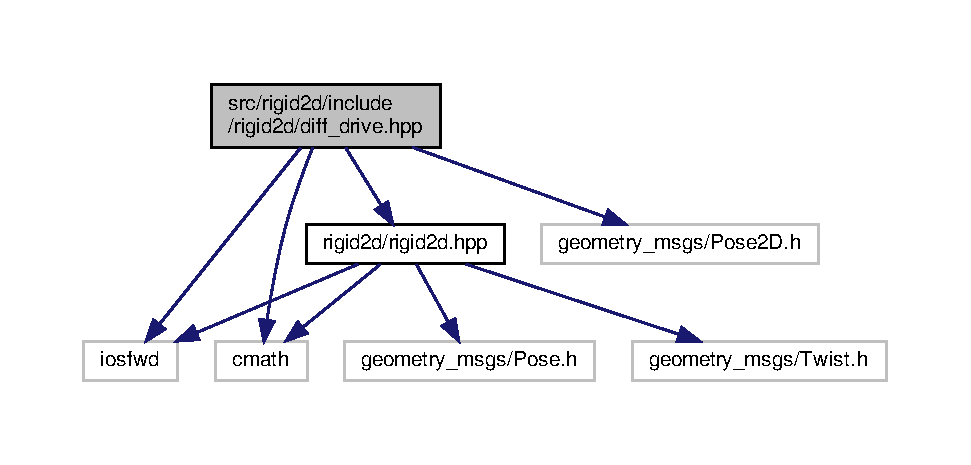
\includegraphics[width=350pt]{diff__drive_8hpp__incl}
\end{center}
\end{figure}
\subsection*{Classes}
\begin{DoxyCompactItemize}
\item 
struct \hyperlink{structrigid2d_1_1WheelVelocities}{rigid2d\+::\+Wheel\+Velocities}
\begin{DoxyCompactList}\small\item\em Desribes desired wheel velocities in radians/s. \end{DoxyCompactList}\item 
class \hyperlink{classrigid2d_1_1DiffDrive}{rigid2d\+::\+Diff\+Drive}
\begin{DoxyCompactList}\small\item\em Implements high level abstraction and tracking of a diff drive robot. \end{DoxyCompactList}\end{DoxyCompactItemize}


\subsection{Detailed Description}
Implements high level abstraction and tracking of a diff drive robot. 


\hypertarget{rigid2d_8hpp}{}\section{src/rigid2d/include/rigid2d/rigid2d.hpp File Reference}
\label{rigid2d_8hpp}\index{src/rigid2d/include/rigid2d/rigid2d.\+hpp@{src/rigid2d/include/rigid2d/rigid2d.\+hpp}}


Library for two-\/dimensional rigid body transformations.  


{\ttfamily \#include $<$iosfwd$>$}\newline
{\ttfamily \#include $<$cmath$>$}\newline
{\ttfamily \#include $<$geometry\+\_\+msgs/\+Pose.\+h$>$}\newline
{\ttfamily \#include $<$geometry\+\_\+msgs/\+Twist.\+h$>$}\newline
Include dependency graph for rigid2d.\+hpp\+:
\nopagebreak
\begin{figure}[H]
\begin{center}
\leavevmode
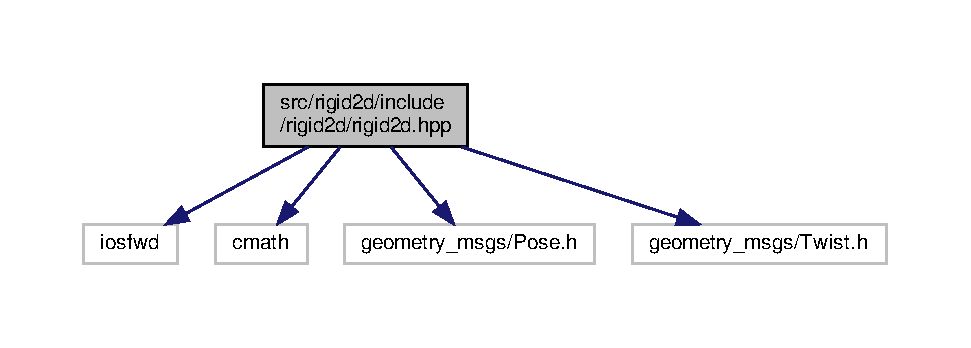
\includegraphics[width=350pt]{rigid2d_8hpp__incl}
\end{center}
\end{figure}
This graph shows which files directly or indirectly include this file\+:
\nopagebreak
\begin{figure}[H]
\begin{center}
\leavevmode
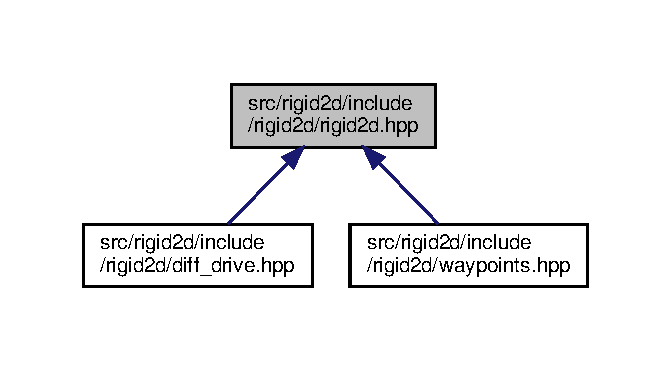
\includegraphics[width=322pt]{rigid2d_8hpp__dep__incl}
\end{center}
\end{figure}
\subsection*{Classes}
\begin{DoxyCompactItemize}
\item 
struct \hyperlink{structrigid2d_1_1Vector2D}{rigid2d\+::\+Vector2D}
\begin{DoxyCompactList}\small\item\em A 2-\/\+Dimensional Vector. \end{DoxyCompactList}\item 
class \hyperlink{classrigid2d_1_1Twist2D}{rigid2d\+::\+Twist2D}
\item 
class \hyperlink{classrigid2d_1_1Transform2D}{rigid2d\+::\+Transform2D}
\begin{DoxyCompactList}\small\item\em a rigid body transformation in 2 dimensions \end{DoxyCompactList}\end{DoxyCompactItemize}
\subsection*{Functions}
\begin{DoxyCompactItemize}
\item 
constexpr bool \hyperlink{rigid2d_8hpp_aa56fa40a409082af8395dbd4e1a25b1b}{rigid2d\+::almost\+\_\+equal} (double d1, double d2, double epsilon=1.\+0e-\/12)
\begin{DoxyCompactList}\small\item\em approximately compare two floating-\/point numbers using an absolute comparison \end{DoxyCompactList}\item 
constexpr double \hyperlink{rigid2d_8hpp_a0366e0678d25f256b74525151b28b1e0}{rigid2d\+::normalize\+\_\+angle} (double rad)
\begin{DoxyCompactList}\small\item\em Maps angle into \mbox{[}-\/pi, pi\mbox{]}. \end{DoxyCompactList}\item 
constexpr double \hyperlink{rigid2d_8hpp_a58a218146f51c0c2454e5fe1a83cb04c}{rigid2d\+::deg2rad} (double deg)
\begin{DoxyCompactList}\small\item\em convert degrees to radians \end{DoxyCompactList}\item 
constexpr double \hyperlink{rigid2d_8hpp_a6883dbf1c0018c962e890754e9d5f62f}{rigid2d\+::rad2deg} (double rad)
\begin{DoxyCompactList}\small\item\em convert radians to degrees \end{DoxyCompactList}\item 
Vector2D \hyperlink{rigid2d_8hpp_a2e41c4314e589a00ba057c387b216666}{rigid2d\+::normalize} (Vector2D orig\+\_\+vector)
\begin{DoxyCompactList}\small\item\em Normalizes a vector to be of unit length. \end{DoxyCompactList}\item 
std\+::ostream \& \hyperlink{rigid2d_8hpp_abadb1659e848f0c3d4ee84943a986495}{rigid2d\+::operator$<$$<$} (std\+::ostream \&os, const Vector2D \&v)
\begin{DoxyCompactList}\small\item\em output a 2 dimensional vector as \mbox{[}xcomponent ycomponent\mbox{]} \end{DoxyCompactList}\item 
bool \hyperlink{rigid2d_8hpp_a88992543be883c665fad3eeb2f286fd2}{rigid2d\+::operator==} (const \hyperlink{classrigid2d_1_1Transform2D}{rigid2d\+::\+Transform2D} \&lhs, const \hyperlink{classrigid2d_1_1Transform2D}{rigid2d\+::\+Transform2D} \&rhs)
\begin{DoxyCompactList}\small\item\em Does comparsion of two Transform2\+Ds This is useful for testing to see if two transforms are equal. \end{DoxyCompactList}\item 
bool \hyperlink{rigid2d_8hpp_ab8185824e983350a0a0749b60462a2a4}{rigid2d\+::operator!=} (const \hyperlink{classrigid2d_1_1Transform2D}{rigid2d\+::\+Transform2D} \&lhs, const \hyperlink{classrigid2d_1_1Transform2D}{rigid2d\+::\+Transform2D} \&rhs)
\begin{DoxyCompactList}\small\item\em Does inequality check of two Transform2\+Ds This is useful for testing to see if two transforms are equal. \end{DoxyCompactList}\item 
bool \hyperlink{rigid2d_8hpp_a493744bb7d92efd8ac941b14ae682658}{rigid2d\+::operator==} (const \hyperlink{structrigid2d_1_1Vector2D}{rigid2d\+::\+Vector2D} \&lhs, const \hyperlink{structrigid2d_1_1Vector2D}{rigid2d\+::\+Vector2D} \&rhs)
\begin{DoxyCompactList}\small\item\em Does comparsion of two Transform2\+Ds This is useful for testing to see if two transforms are equal. \end{DoxyCompactList}\item 
bool \hyperlink{rigid2d_8hpp_a2652463319dbf1c72e96995cb4b317af}{rigid2d\+::operator!=} (const \hyperlink{structrigid2d_1_1Vector2D}{rigid2d\+::\+Vector2D} \&lhs, const \hyperlink{structrigid2d_1_1Vector2D}{rigid2d\+::\+Vector2D} \&rhs)
\begin{DoxyCompactList}\small\item\em Does inequality check of two Transform2\+Ds This is useful for testing to see if two transforms are equal. \end{DoxyCompactList}\item 
std\+::ostream \& \hyperlink{rigid2d_8hpp_a7f6157a71a99749b32338b98745547fc}{rigid2d\+::operator$<$$<$} (std\+::ostream \&os, const Twist2D \&tw)
\begin{DoxyCompactList}\small\item\em Print a human readable description of the twist. \end{DoxyCompactList}\item 
std\+::istream \& \hyperlink{rigid2d_8hpp_ac5891668753fe470ad93b6834c109d25}{rigid2d\+::operator$>$$>$} (std\+::istream \&is, Twist2D \&tw)
\begin{DoxyCompactList}\small\item\em Read in a Twist2d from the user. \end{DoxyCompactList}\item 
std\+::ostream \& \hyperlink{rigid2d_8hpp_a88d49617eb8d576d5ad73fcf0f8b8694}{rigid2d\+::operator$<$$<$} (std\+::ostream \&os, const Transform2D \&tf)
\begin{DoxyCompactList}\small\item\em Print a human readable description of the \hyperlink{classrigid2d_1_1Transform2D}{Transform2D}. \end{DoxyCompactList}\item 
std\+::istream \& \hyperlink{rigid2d_8hpp_ac36117d4cb21edf2a7e0a0790dcdc79e}{rigid2d\+::operator$>$$>$} (std\+::istream \&is, Transform2D \&tf)
\begin{DoxyCompactList}\small\item\em Reads in a \hyperlink{classrigid2d_1_1Transform2D}{Transform2D} from the user. \end{DoxyCompactList}\item 
Transform2D \hyperlink{rigid2d_8hpp_ae2da06dacbf1c4f34a88cb0f6cd29873}{rigid2d\+::operator$\ast$} (const Transform2D \&lhs, const Transform2D \&rhs)
\begin{DoxyCompactList}\small\item\em Compose two transformations together and return the result. \end{DoxyCompactList}\item 
bool \hyperlink{rigid2d_8hpp_aa06fe1740b7b598dba1d76811f9b63d6}{rigid2d\+::operator==} (const \hyperlink{classrigid2d_1_1Twist2D}{rigid2d\+::\+Twist2D} \&lhs, const \hyperlink{classrigid2d_1_1Twist2D}{rigid2d\+::\+Twist2D} \&rhs)
\begin{DoxyCompactList}\small\item\em Does comparsion of two Transform2\+Ds This is useful for testing to see if two transforms are equal. \end{DoxyCompactList}\item 
bool \hyperlink{rigid2d_8hpp_a10a57a12a8268b425d53fe21466e185d}{rigid2d\+::operator!=} (const \hyperlink{classrigid2d_1_1Twist2D}{rigid2d\+::\+Twist2D} \&lhs, const \hyperlink{classrigid2d_1_1Twist2D}{rigid2d\+::\+Twist2D} \&rhs)
\begin{DoxyCompactList}\small\item\em Does inequality check of two Transform2\+Ds. \end{DoxyCompactList}\item 
Vector2D \hyperlink{rigid2d_8hpp_a1084041bae612af1fce089c1ef989c95}{rigid2d\+::operator+} (const \hyperlink{structrigid2d_1_1Vector2D}{rigid2d\+::\+Vector2D} \&lhs, const \hyperlink{structrigid2d_1_1Vector2D}{rigid2d\+::\+Vector2D} \&rhs)
\begin{DoxyCompactList}\small\item\em Perform vector addition. \end{DoxyCompactList}\item 
Vector2D \hyperlink{rigid2d_8hpp_afd79e8ba183a69b41c2d106dbe37b653}{rigid2d\+::operator+=} (\hyperlink{structrigid2d_1_1Vector2D}{rigid2d\+::\+Vector2D} \&lhs, const \hyperlink{structrigid2d_1_1Vector2D}{rigid2d\+::\+Vector2D} \&rhs)
\begin{DoxyCompactList}\small\item\em Perform vector addition. \end{DoxyCompactList}\item 
Vector2D \hyperlink{rigid2d_8hpp_a301b20eac1e0ba6e80fe6f12f45f69d1}{rigid2d\+::operator-\/} (const \hyperlink{structrigid2d_1_1Vector2D}{rigid2d\+::\+Vector2D} \&lhs, const \hyperlink{structrigid2d_1_1Vector2D}{rigid2d\+::\+Vector2D} \&rhs)
\begin{DoxyCompactList}\small\item\em Perform vector subtraction. \end{DoxyCompactList}\item 
Vector2D \hyperlink{rigid2d_8hpp_a6f9ed63b4a375d17d2f7b03a68939f23}{rigid2d\+::operator-\/=} (const \hyperlink{structrigid2d_1_1Vector2D}{rigid2d\+::\+Vector2D} \&lhs, const \hyperlink{structrigid2d_1_1Vector2D}{rigid2d\+::\+Vector2D} \&rhs)
\begin{DoxyCompactList}\small\item\em Perform vector subtraction. \end{DoxyCompactList}\item 
Vector2D \hyperlink{rigid2d_8hpp_a64ca95f74e975c06d61a91e49f3eb80e}{rigid2d\+::operator$\ast$} (const \hyperlink{structrigid2d_1_1Vector2D}{rigid2d\+::\+Vector2D} \&lhs, const double \&rhs)
\begin{DoxyCompactList}\small\item\em Perform scalar multiplication of a vector. \end{DoxyCompactList}\item 
Vector2D \hyperlink{rigid2d_8hpp_aad96eb34c174fe56f2b9292368e084b8}{rigid2d\+::operator$\ast$} (const double \&rhs, const \hyperlink{structrigid2d_1_1Vector2D}{rigid2d\+::\+Vector2D} \&lhs)
\begin{DoxyCompactList}\small\item\em Perform scalar multiplication of a vector. \end{DoxyCompactList}\item 
Vector2D \hyperlink{rigid2d_8hpp_a77f0b7e25440a4d2807568f9afab668a}{rigid2d\+::operator$\ast$=} (\hyperlink{structrigid2d_1_1Vector2D}{rigid2d\+::\+Vector2D} \&lhs, const double \&rhs)
\begin{DoxyCompactList}\small\item\em Perform scalar multiplication of a vector. \end{DoxyCompactList}\item 
double \hyperlink{rigid2d_8hpp_a32f910a0237fae325f5f87b654c36f95}{rigid2d\+::length} (const \hyperlink{structrigid2d_1_1Vector2D}{rigid2d\+::\+Vector2D} \&vector)
\begin{DoxyCompactList}\small\item\em Compute the length of a vector. \end{DoxyCompactList}\item 
double \hyperlink{rigid2d_8hpp_a8d5c38db29872911eaac1ddaea12748d}{rigid2d\+::angle} (const \hyperlink{structrigid2d_1_1Vector2D}{rigid2d\+::\+Vector2D} \&vector)
\begin{DoxyCompactList}\small\item\em Compute and the angle of a vector. \end{DoxyCompactList}\item 
double \hyperlink{rigid2d_8hpp_ad8a51427dacefa3c96594a7f867436ee}{rigid2d\+::distance} (const \hyperlink{structrigid2d_1_1Vector2D}{rigid2d\+::\+Vector2D} \&lhs, const \hyperlink{structrigid2d_1_1Vector2D}{rigid2d\+::\+Vector2D} \&rhs)
\begin{DoxyCompactList}\small\item\em Compute the distance between two vectors. \end{DoxyCompactList}\item 
Twist2D \hyperlink{rigid2d_8hpp_aa2d04bfe16de71b629f59c6bd1423504}{rigid2d\+::convert3\+D\+To2D} (geometry\+\_\+msgs\+::\+Twist twist)
\begin{DoxyCompactList}\small\item\em Convert the geometry\+\_\+msgs\+::\+Twist object to a \hyperlink{classrigid2d_1_1Twist2D}{rigid2d\+::\+Twist2D} object. \end{DoxyCompactList}\end{DoxyCompactItemize}
\subsection*{Variables}
\begin{DoxyCompactItemize}
\item 
\mbox{\Hypertarget{rigid2d_8hpp_af68d2597a40a3021e2c66d1c23019952}\label{rigid2d_8hpp_af68d2597a40a3021e2c66d1c23019952}} 
constexpr double \hyperlink{rigid2d_8hpp_af68d2597a40a3021e2c66d1c23019952}{rigid2d\+::\+PI} = 3.\+14159265358979323846
\begin{DoxyCompactList}\small\item\em PI. Not in C++ standard until C++20. \end{DoxyCompactList}\end{DoxyCompactItemize}


\subsection{Detailed Description}
Library for two-\/dimensional rigid body transformations. 



\subsection{Function Documentation}
\mbox{\Hypertarget{rigid2d_8hpp_file_aa56fa40a409082af8395dbd4e1a25b1b}\label{rigid2d_8hpp_file_aa56fa40a409082af8395dbd4e1a25b1b}} 
\index{rigid2d.\+hpp@{rigid2d.\+hpp}!almost\+\_\+equal@{almost\+\_\+equal}}
\index{almost\+\_\+equal@{almost\+\_\+equal}!rigid2d.\+hpp@{rigid2d.\+hpp}}
\subsubsection{\texorpdfstring{almost\+\_\+equal()}{almost\_equal()}}
{\footnotesize\ttfamily constexpr bool rigid2d\+::almost\+\_\+equal (\begin{DoxyParamCaption}\item[{double}]{d1,  }\item[{double}]{d2,  }\item[{double}]{epsilon = {\ttfamily 1.0e-\/12} }\end{DoxyParamCaption})}



approximately compare two floating-\/point numbers using an absolute comparison 


\begin{DoxyParams}{Parameters}
{\em d1} & -\/ a number to compare \\
\hline
{\em d2} & -\/ a second number to compare \\
\hline
{\em epsilon} & -\/ absolute threshold required for equality \\
\hline
\end{DoxyParams}
\begin{DoxyReturn}{Returns}
true if abs(d1 -\/ d2) $<$ epsilon 
\end{DoxyReturn}
\mbox{\Hypertarget{rigid2d_8hpp_file_a8d5c38db29872911eaac1ddaea12748d}\label{rigid2d_8hpp_file_a8d5c38db29872911eaac1ddaea12748d}} 
\index{rigid2d.\+hpp@{rigid2d.\+hpp}!angle@{angle}}
\index{angle@{angle}!rigid2d.\+hpp@{rigid2d.\+hpp}}
\subsubsection{\texorpdfstring{angle()}{angle()}}
{\footnotesize\ttfamily double rigid2d\+::angle (\begin{DoxyParamCaption}\item[{const \hyperlink{structrigid2d_1_1Vector2D}{rigid2d\+::\+Vector2D} \&}]{vector }\end{DoxyParamCaption})}



Compute and the angle of a vector. 


\begin{DoxyParams}{Parameters}
{\em vector} & -\/ the vector whose angle we are computing \\
\hline
\end{DoxyParams}
\begin{DoxyReturn}{Returns}
the angle in radians 
\end{DoxyReturn}
\mbox{\Hypertarget{rigid2d_8hpp_file_aa2d04bfe16de71b629f59c6bd1423504}\label{rigid2d_8hpp_file_aa2d04bfe16de71b629f59c6bd1423504}} 
\index{rigid2d.\+hpp@{rigid2d.\+hpp}!convert3\+D\+To2D@{convert3\+D\+To2D}}
\index{convert3\+D\+To2D@{convert3\+D\+To2D}!rigid2d.\+hpp@{rigid2d.\+hpp}}
\subsubsection{\texorpdfstring{convert3\+D\+To2\+D()}{convert3DTo2D()}}
{\footnotesize\ttfamily Twist2D rigid2d\+::convert3\+D\+To2D (\begin{DoxyParamCaption}\item[{geometry\+\_\+msgs\+::\+Twist}]{twist }\end{DoxyParamCaption})}



Convert the geometry\+\_\+msgs\+::\+Twist object to a \hyperlink{classrigid2d_1_1Twist2D}{rigid2d\+::\+Twist2D} object. 


\begin{DoxyParams}{Parameters}
{\em twist} & -\/ the twist in R\+OS format \\
\hline
\end{DoxyParams}
\begin{DoxyReturn}{Returns}
the twist in rigid2D format 
\end{DoxyReturn}
\mbox{\Hypertarget{rigid2d_8hpp_file_a58a218146f51c0c2454e5fe1a83cb04c}\label{rigid2d_8hpp_file_a58a218146f51c0c2454e5fe1a83cb04c}} 
\index{rigid2d.\+hpp@{rigid2d.\+hpp}!deg2rad@{deg2rad}}
\index{deg2rad@{deg2rad}!rigid2d.\+hpp@{rigid2d.\+hpp}}
\subsubsection{\texorpdfstring{deg2rad()}{deg2rad()}}
{\footnotesize\ttfamily constexpr double rigid2d\+::deg2rad (\begin{DoxyParamCaption}\item[{double}]{deg }\end{DoxyParamCaption})}



convert degrees to radians 


\begin{DoxyParams}{Parameters}
{\em deg} & -\/ angle in degrees \\
\hline
\end{DoxyParams}
\begin{DoxyReturn}{Returns}
the angle in radians 
\end{DoxyReturn}
\mbox{\Hypertarget{rigid2d_8hpp_file_ad8a51427dacefa3c96594a7f867436ee}\label{rigid2d_8hpp_file_ad8a51427dacefa3c96594a7f867436ee}} 
\index{rigid2d.\+hpp@{rigid2d.\+hpp}!distance@{distance}}
\index{distance@{distance}!rigid2d.\+hpp@{rigid2d.\+hpp}}
\subsubsection{\texorpdfstring{distance()}{distance()}}
{\footnotesize\ttfamily double rigid2d\+::distance (\begin{DoxyParamCaption}\item[{const \hyperlink{structrigid2d_1_1Vector2D}{rigid2d\+::\+Vector2D} \&}]{lhs,  }\item[{const \hyperlink{structrigid2d_1_1Vector2D}{rigid2d\+::\+Vector2D} \&}]{rhs }\end{DoxyParamCaption})}



Compute the distance between two vectors. 


\begin{DoxyParams}{Parameters}
{\em lhs} & -\/ the left hand side vector \\
\hline
{\em rhs} & -\/ the right hand side vector \\
\hline
\end{DoxyParams}
\begin{DoxyReturn}{Returns}
the distance between two vectors 
\end{DoxyReturn}
\mbox{\Hypertarget{rigid2d_8hpp_file_a32f910a0237fae325f5f87b654c36f95}\label{rigid2d_8hpp_file_a32f910a0237fae325f5f87b654c36f95}} 
\index{rigid2d.\+hpp@{rigid2d.\+hpp}!length@{length}}
\index{length@{length}!rigid2d.\+hpp@{rigid2d.\+hpp}}
\subsubsection{\texorpdfstring{length()}{length()}}
{\footnotesize\ttfamily double rigid2d\+::length (\begin{DoxyParamCaption}\item[{const \hyperlink{structrigid2d_1_1Vector2D}{rigid2d\+::\+Vector2D} \&}]{vector }\end{DoxyParamCaption})}



Compute the length of a vector. 


\begin{DoxyParams}{Parameters}
{\em vector} & -\/ the vector whose length we compute \\
\hline
\end{DoxyParams}
\begin{DoxyReturn}{Returns}
the length of the vector 
\end{DoxyReturn}
\mbox{\Hypertarget{rigid2d_8hpp_file_a2e41c4314e589a00ba057c387b216666}\label{rigid2d_8hpp_file_a2e41c4314e589a00ba057c387b216666}} 
\index{rigid2d.\+hpp@{rigid2d.\+hpp}!normalize@{normalize}}
\index{normalize@{normalize}!rigid2d.\+hpp@{rigid2d.\+hpp}}
\subsubsection{\texorpdfstring{normalize()}{normalize()}}
{\footnotesize\ttfamily Vector2D rigid2d\+::normalize (\begin{DoxyParamCaption}\item[{\hyperlink{structrigid2d_1_1Vector2D}{Vector2D}}]{orig\+\_\+vector }\end{DoxyParamCaption})}



Normalizes a vector to be of unit length. 


\begin{DoxyParams}{Parameters}
{\em orig\+\_\+vector} & is the vector to be normalized \\
\hline
\end{DoxyParams}
\begin{DoxyReturn}{Returns}
the normalized vector 
\end{DoxyReturn}
\mbox{\Hypertarget{rigid2d_8hpp_file_a0366e0678d25f256b74525151b28b1e0}\label{rigid2d_8hpp_file_a0366e0678d25f256b74525151b28b1e0}} 
\index{rigid2d.\+hpp@{rigid2d.\+hpp}!normalize\+\_\+angle@{normalize\+\_\+angle}}
\index{normalize\+\_\+angle@{normalize\+\_\+angle}!rigid2d.\+hpp@{rigid2d.\+hpp}}
\subsubsection{\texorpdfstring{normalize\+\_\+angle()}{normalize\_angle()}}
{\footnotesize\ttfamily constexpr double rigid2d\+::normalize\+\_\+angle (\begin{DoxyParamCaption}\item[{double}]{rad }\end{DoxyParamCaption})}



Maps angle into \mbox{[}-\/pi, pi\mbox{]}. 


\begin{DoxyParams}{Parameters}
{\em rad} & is the original angle in radians \\
\hline
\end{DoxyParams}
\begin{DoxyReturn}{Returns}
the normalized angle 
\end{DoxyReturn}
\mbox{\Hypertarget{rigid2d_8hpp_file_ab8185824e983350a0a0749b60462a2a4}\label{rigid2d_8hpp_file_ab8185824e983350a0a0749b60462a2a4}} 
\index{rigid2d.\+hpp@{rigid2d.\+hpp}!operator"!=@{operator"!=}}
\index{operator"!=@{operator"!=}!rigid2d.\+hpp@{rigid2d.\+hpp}}
\subsubsection{\texorpdfstring{operator"!=()}{operator!=()}\hspace{0.1cm}{\footnotesize\ttfamily [1/3]}}
{\footnotesize\ttfamily bool rigid2d\+::operator!= (\begin{DoxyParamCaption}\item[{const \hyperlink{classrigid2d_1_1Transform2D}{rigid2d\+::\+Transform2D} \&}]{lhs,  }\item[{const \hyperlink{classrigid2d_1_1Transform2D}{rigid2d\+::\+Transform2D} \&}]{rhs }\end{DoxyParamCaption})}



Does inequality check of two Transform2\+Ds This is useful for testing to see if two transforms are equal. 


\begin{DoxyParams}{Parameters}
{\em lhs} & -\/ the left hand side Transform2D \\
\hline
{\em rhs} & -\/ the right hand side Transform2D \\
\hline
\end{DoxyParams}
\begin{DoxyReturn}{Returns}
false if the two S\+E(2) are equal (within small tolerance), true otherwise 
\end{DoxyReturn}
\mbox{\Hypertarget{rigid2d_8hpp_file_a2652463319dbf1c72e96995cb4b317af}\label{rigid2d_8hpp_file_a2652463319dbf1c72e96995cb4b317af}} 
\index{rigid2d.\+hpp@{rigid2d.\+hpp}!operator"!=@{operator"!=}}
\index{operator"!=@{operator"!=}!rigid2d.\+hpp@{rigid2d.\+hpp}}
\subsubsection{\texorpdfstring{operator"!=()}{operator!=()}\hspace{0.1cm}{\footnotesize\ttfamily [2/3]}}
{\footnotesize\ttfamily bool rigid2d\+::operator!= (\begin{DoxyParamCaption}\item[{const \hyperlink{structrigid2d_1_1Vector2D}{rigid2d\+::\+Vector2D} \&}]{lhs,  }\item[{const \hyperlink{structrigid2d_1_1Vector2D}{rigid2d\+::\+Vector2D} \&}]{rhs }\end{DoxyParamCaption})}



Does inequality check of two Transform2\+Ds This is useful for testing to see if two transforms are equal. 


\begin{DoxyParams}{Parameters}
{\em lhs} & -\/ the left hand side Transform2D \\
\hline
{\em rhs} & -\/ the right hand side Transform2D \\
\hline
\end{DoxyParams}
\begin{DoxyReturn}{Returns}
false if the two S\+E(2) are equal (within small tolerance), true otherwise 
\end{DoxyReturn}
\mbox{\Hypertarget{rigid2d_8hpp_file_a10a57a12a8268b425d53fe21466e185d}\label{rigid2d_8hpp_file_a10a57a12a8268b425d53fe21466e185d}} 
\index{rigid2d.\+hpp@{rigid2d.\+hpp}!operator"!=@{operator"!=}}
\index{operator"!=@{operator"!=}!rigid2d.\+hpp@{rigid2d.\+hpp}}
\subsubsection{\texorpdfstring{operator"!=()}{operator!=()}\hspace{0.1cm}{\footnotesize\ttfamily [3/3]}}
{\footnotesize\ttfamily bool rigid2d\+::operator!= (\begin{DoxyParamCaption}\item[{const \hyperlink{classrigid2d_1_1Twist2D}{rigid2d\+::\+Twist2D} \&}]{lhs,  }\item[{const \hyperlink{classrigid2d_1_1Twist2D}{rigid2d\+::\+Twist2D} \&}]{rhs }\end{DoxyParamCaption})}



Does inequality check of two Transform2\+Ds. 


\begin{DoxyParams}{Parameters}
{\em lhs} & -\/ the left hand side Transform2D \\
\hline
{\em rhs} & -\/ the right hand side Transform2D \\
\hline
\end{DoxyParams}
\begin{DoxyReturn}{Returns}
false if the two S\+E(2) are equal (within small tolerance), true otherwise 
\end{DoxyReturn}
\mbox{\Hypertarget{rigid2d_8hpp_file_ae2da06dacbf1c4f34a88cb0f6cd29873}\label{rigid2d_8hpp_file_ae2da06dacbf1c4f34a88cb0f6cd29873}} 
\index{rigid2d.\+hpp@{rigid2d.\+hpp}!operator$\ast$@{operator$\ast$}}
\index{operator$\ast$@{operator$\ast$}!rigid2d.\+hpp@{rigid2d.\+hpp}}
\subsubsection{\texorpdfstring{operator$\ast$()}{operator*()}\hspace{0.1cm}{\footnotesize\ttfamily [1/3]}}
{\footnotesize\ttfamily Transform2D rigid2d\+::operator$\ast$ (\begin{DoxyParamCaption}\item[{const \hyperlink{classrigid2d_1_1Transform2D}{Transform2D} \&}]{lhs,  }\item[{const \hyperlink{classrigid2d_1_1Transform2D}{Transform2D} \&}]{rhs }\end{DoxyParamCaption})}



Compose two transformations together and return the result. 


\begin{DoxyParams}{Parameters}
{\em lhs} & -\/ the left hand side transformation \\
\hline
{\em rhs} & -\/ the right hand side transformation Note\+: A 2D transformation matrix can be stored with only c\+Theta, s\+Theta, x, and y. There\textquotesingle{}s no need to multiply the entire matrix or store the entire matrix \\
\hline
\end{DoxyParams}
\begin{DoxyReturn}{Returns}
the composition of the two transformations 
\end{DoxyReturn}
\mbox{\Hypertarget{rigid2d_8hpp_file_a64ca95f74e975c06d61a91e49f3eb80e}\label{rigid2d_8hpp_file_a64ca95f74e975c06d61a91e49f3eb80e}} 
\index{rigid2d.\+hpp@{rigid2d.\+hpp}!operator$\ast$@{operator$\ast$}}
\index{operator$\ast$@{operator$\ast$}!rigid2d.\+hpp@{rigid2d.\+hpp}}
\subsubsection{\texorpdfstring{operator$\ast$()}{operator*()}\hspace{0.1cm}{\footnotesize\ttfamily [2/3]}}
{\footnotesize\ttfamily Vector2D rigid2d\+::operator$\ast$ (\begin{DoxyParamCaption}\item[{const \hyperlink{structrigid2d_1_1Vector2D}{rigid2d\+::\+Vector2D} \&}]{lhs,  }\item[{const double \&}]{rhs }\end{DoxyParamCaption})}



Perform scalar multiplication of a vector. 


\begin{DoxyParams}{Parameters}
{\em lhs} & -\/ the left hand side vector \\
\hline
{\em rhs} & -\/ the scalar multiplier \\
\hline
\end{DoxyParams}
\begin{DoxyReturn}{Returns}
the result of a scalar multiply of a vector 
\end{DoxyReturn}
\mbox{\Hypertarget{rigid2d_8hpp_file_aad96eb34c174fe56f2b9292368e084b8}\label{rigid2d_8hpp_file_aad96eb34c174fe56f2b9292368e084b8}} 
\index{rigid2d.\+hpp@{rigid2d.\+hpp}!operator$\ast$@{operator$\ast$}}
\index{operator$\ast$@{operator$\ast$}!rigid2d.\+hpp@{rigid2d.\+hpp}}
\subsubsection{\texorpdfstring{operator$\ast$()}{operator*()}\hspace{0.1cm}{\footnotesize\ttfamily [3/3]}}
{\footnotesize\ttfamily Vector2D rigid2d\+::operator$\ast$ (\begin{DoxyParamCaption}\item[{const double \&}]{rhs,  }\item[{const \hyperlink{structrigid2d_1_1Vector2D}{rigid2d\+::\+Vector2D} \&}]{lhs }\end{DoxyParamCaption})}



Perform scalar multiplication of a vector. 


\begin{DoxyParams}{Parameters}
{\em rhs} & -\/ the scalar multiplier \\
\hline
{\em lhs} & -\/ the vector \\
\hline
\end{DoxyParams}
\begin{DoxyReturn}{Returns}
the result of a scalar multiply of the vector 
\end{DoxyReturn}
\mbox{\Hypertarget{rigid2d_8hpp_file_a77f0b7e25440a4d2807568f9afab668a}\label{rigid2d_8hpp_file_a77f0b7e25440a4d2807568f9afab668a}} 
\index{rigid2d.\+hpp@{rigid2d.\+hpp}!operator$\ast$=@{operator$\ast$=}}
\index{operator$\ast$=@{operator$\ast$=}!rigid2d.\+hpp@{rigid2d.\+hpp}}
\subsubsection{\texorpdfstring{operator$\ast$=()}{operator*=()}}
{\footnotesize\ttfamily Vector2D rigid2d\+::operator$\ast$= (\begin{DoxyParamCaption}\item[{\hyperlink{structrigid2d_1_1Vector2D}{rigid2d\+::\+Vector2D} \&}]{lhs,  }\item[{const double \&}]{rhs }\end{DoxyParamCaption})}



Perform scalar multiplication of a vector. 


\begin{DoxyParams}{Parameters}
{\em lhs} & -\/ the left hand side vector \\
\hline
{\em rhs} & -\/ the right hand side scalar multiplier \\
\hline
\end{DoxyParams}
\begin{DoxyReturn}{Returns}
the result 
\end{DoxyReturn}
\mbox{\Hypertarget{rigid2d_8hpp_file_a1084041bae612af1fce089c1ef989c95}\label{rigid2d_8hpp_file_a1084041bae612af1fce089c1ef989c95}} 
\index{rigid2d.\+hpp@{rigid2d.\+hpp}!operator+@{operator+}}
\index{operator+@{operator+}!rigid2d.\+hpp@{rigid2d.\+hpp}}
\subsubsection{\texorpdfstring{operator+()}{operator+()}}
{\footnotesize\ttfamily Vector2D rigid2d\+::operator+ (\begin{DoxyParamCaption}\item[{const \hyperlink{structrigid2d_1_1Vector2D}{rigid2d\+::\+Vector2D} \&}]{lhs,  }\item[{const \hyperlink{structrigid2d_1_1Vector2D}{rigid2d\+::\+Vector2D} \&}]{rhs }\end{DoxyParamCaption})}



Perform vector addition. 


\begin{DoxyParams}{Parameters}
{\em lhs} & -\/ the left hand side vector \\
\hline
{\em rhs} & -\/ the right hand side vector \\
\hline
\end{DoxyParams}
\begin{DoxyReturn}{Returns}
the result of the vector addition 
\end{DoxyReturn}
\mbox{\Hypertarget{rigid2d_8hpp_file_afd79e8ba183a69b41c2d106dbe37b653}\label{rigid2d_8hpp_file_afd79e8ba183a69b41c2d106dbe37b653}} 
\index{rigid2d.\+hpp@{rigid2d.\+hpp}!operator+=@{operator+=}}
\index{operator+=@{operator+=}!rigid2d.\+hpp@{rigid2d.\+hpp}}
\subsubsection{\texorpdfstring{operator+=()}{operator+=()}}
{\footnotesize\ttfamily Vector2D rigid2d\+::operator+= (\begin{DoxyParamCaption}\item[{\hyperlink{structrigid2d_1_1Vector2D}{rigid2d\+::\+Vector2D} \&}]{lhs,  }\item[{const \hyperlink{structrigid2d_1_1Vector2D}{rigid2d\+::\+Vector2D} \&}]{rhs }\end{DoxyParamCaption})}



Perform vector addition. 


\begin{DoxyParams}{Parameters}
{\em lhs} & -\/ the left hand side vector \\
\hline
{\em rhs} & -\/ the right hand side vector \\
\hline
\end{DoxyParams}
\begin{DoxyReturn}{Returns}
the result of the vector addition 
\end{DoxyReturn}
\mbox{\Hypertarget{rigid2d_8hpp_file_a301b20eac1e0ba6e80fe6f12f45f69d1}\label{rigid2d_8hpp_file_a301b20eac1e0ba6e80fe6f12f45f69d1}} 
\index{rigid2d.\+hpp@{rigid2d.\+hpp}!operator-\/@{operator-\/}}
\index{operator-\/@{operator-\/}!rigid2d.\+hpp@{rigid2d.\+hpp}}
\subsubsection{\texorpdfstring{operator-\/()}{operator-()}}
{\footnotesize\ttfamily Vector2D rigid2d\+::operator-\/ (\begin{DoxyParamCaption}\item[{const \hyperlink{structrigid2d_1_1Vector2D}{rigid2d\+::\+Vector2D} \&}]{lhs,  }\item[{const \hyperlink{structrigid2d_1_1Vector2D}{rigid2d\+::\+Vector2D} \&}]{rhs }\end{DoxyParamCaption})}



Perform vector subtraction. 


\begin{DoxyParams}{Parameters}
{\em lhs} & -\/ the left hand side vector \\
\hline
{\em rhs} & -\/ right hand side vector \\
\hline
\end{DoxyParams}
\begin{DoxyReturn}{Returns}
the result of the vector subtraction 
\end{DoxyReturn}
\mbox{\Hypertarget{rigid2d_8hpp_file_a6f9ed63b4a375d17d2f7b03a68939f23}\label{rigid2d_8hpp_file_a6f9ed63b4a375d17d2f7b03a68939f23}} 
\index{rigid2d.\+hpp@{rigid2d.\+hpp}!operator-\/=@{operator-\/=}}
\index{operator-\/=@{operator-\/=}!rigid2d.\+hpp@{rigid2d.\+hpp}}
\subsubsection{\texorpdfstring{operator-\/=()}{operator-=()}}
{\footnotesize\ttfamily Vector2D rigid2d\+::operator-\/= (\begin{DoxyParamCaption}\item[{const \hyperlink{structrigid2d_1_1Vector2D}{rigid2d\+::\+Vector2D} \&}]{lhs,  }\item[{const \hyperlink{structrigid2d_1_1Vector2D}{rigid2d\+::\+Vector2D} \&}]{rhs }\end{DoxyParamCaption})}



Perform vector subtraction. 


\begin{DoxyParams}{Parameters}
{\em lhs} & -\/ the left hand side vector \\
\hline
{\em rhs} & -\/ the right hand side vector \\
\hline
\end{DoxyParams}
\begin{DoxyReturn}{Returns}
the result of the vector subtraction 
\end{DoxyReturn}
\mbox{\Hypertarget{rigid2d_8hpp_file_abadb1659e848f0c3d4ee84943a986495}\label{rigid2d_8hpp_file_abadb1659e848f0c3d4ee84943a986495}} 
\index{rigid2d.\+hpp@{rigid2d.\+hpp}!operator$<$$<$@{operator$<$$<$}}
\index{operator$<$$<$@{operator$<$$<$}!rigid2d.\+hpp@{rigid2d.\+hpp}}
\subsubsection{\texorpdfstring{operator$<$$<$()}{operator<<()}\hspace{0.1cm}{\footnotesize\ttfamily [1/3]}}
{\footnotesize\ttfamily std\+::ostream\& rigid2d\+::operator$<$$<$ (\begin{DoxyParamCaption}\item[{std\+::ostream \&}]{os,  }\item[{const \hyperlink{structrigid2d_1_1Vector2D}{Vector2D} \&}]{v }\end{DoxyParamCaption})}



output a 2 dimensional vector as \mbox{[}xcomponent ycomponent\mbox{]} 


\begin{DoxyParams}{Parameters}
{\em os} & -\/ stream to output to \\
\hline
{\em v} & -\/ the vector to print \\
\hline
\end{DoxyParams}
\begin{DoxyReturn}{Returns}
the output stream 
\end{DoxyReturn}
\mbox{\Hypertarget{rigid2d_8hpp_file_a7f6157a71a99749b32338b98745547fc}\label{rigid2d_8hpp_file_a7f6157a71a99749b32338b98745547fc}} 
\index{rigid2d.\+hpp@{rigid2d.\+hpp}!operator$<$$<$@{operator$<$$<$}}
\index{operator$<$$<$@{operator$<$$<$}!rigid2d.\+hpp@{rigid2d.\+hpp}}
\subsubsection{\texorpdfstring{operator$<$$<$()}{operator<<()}\hspace{0.1cm}{\footnotesize\ttfamily [2/3]}}
{\footnotesize\ttfamily std\+::ostream\& rigid2d\+::operator$<$$<$ (\begin{DoxyParamCaption}\item[{std\+::ostream \&}]{os,  }\item[{const \hyperlink{classrigid2d_1_1Twist2D}{Twist2D} \&}]{tw }\end{DoxyParamCaption})}



Print a human readable description of the twist. 


\begin{DoxyParams}{Parameters}
{\em os} & -\/ the output stream \\
\hline
{\em tw} & -\/ the twist we are describing \\
\hline
\end{DoxyParams}
\begin{DoxyReturn}{Returns}
the output stream 
\end{DoxyReturn}
\mbox{\Hypertarget{rigid2d_8hpp_file_a88d49617eb8d576d5ad73fcf0f8b8694}\label{rigid2d_8hpp_file_a88d49617eb8d576d5ad73fcf0f8b8694}} 
\index{rigid2d.\+hpp@{rigid2d.\+hpp}!operator$<$$<$@{operator$<$$<$}}
\index{operator$<$$<$@{operator$<$$<$}!rigid2d.\+hpp@{rigid2d.\+hpp}}
\subsubsection{\texorpdfstring{operator$<$$<$()}{operator<<()}\hspace{0.1cm}{\footnotesize\ttfamily [3/3]}}
{\footnotesize\ttfamily std\+::ostream\& rigid2d\+::operator$<$$<$ (\begin{DoxyParamCaption}\item[{std\+::ostream \&}]{os,  }\item[{const \hyperlink{classrigid2d_1_1Transform2D}{Transform2D} \&}]{tf }\end{DoxyParamCaption})}



Print a human readable description of the Transform2D. 

Print a human readable description of the twist.


\begin{DoxyParams}{Parameters}
{\em os} & -\/ the output stream \\
\hline
{\em tf} & -\/ the Transform2D we are describing \\
\hline
\end{DoxyParams}
\begin{DoxyReturn}{Returns}
the output stream 
\end{DoxyReturn}
\mbox{\Hypertarget{rigid2d_8hpp_file_a88992543be883c665fad3eeb2f286fd2}\label{rigid2d_8hpp_file_a88992543be883c665fad3eeb2f286fd2}} 
\index{rigid2d.\+hpp@{rigid2d.\+hpp}!operator==@{operator==}}
\index{operator==@{operator==}!rigid2d.\+hpp@{rigid2d.\+hpp}}
\subsubsection{\texorpdfstring{operator==()}{operator==()}\hspace{0.1cm}{\footnotesize\ttfamily [1/3]}}
{\footnotesize\ttfamily bool rigid2d\+::operator== (\begin{DoxyParamCaption}\item[{const \hyperlink{classrigid2d_1_1Transform2D}{rigid2d\+::\+Transform2D} \&}]{lhs,  }\item[{const \hyperlink{classrigid2d_1_1Transform2D}{rigid2d\+::\+Transform2D} \&}]{rhs }\end{DoxyParamCaption})}



Does comparsion of two Transform2\+Ds This is useful for testing to see if two transforms are equal. 


\begin{DoxyParams}{Parameters}
{\em lhs} & -\/ the left hand side Transform2D \\
\hline
{\em rhs} & -\/ the right hand side Transform2D \\
\hline
\end{DoxyParams}
\begin{DoxyReturn}{Returns}
true if two S\+E(2) are equal (within small tolerance), false otherwise 
\end{DoxyReturn}
\mbox{\Hypertarget{rigid2d_8hpp_file_a493744bb7d92efd8ac941b14ae682658}\label{rigid2d_8hpp_file_a493744bb7d92efd8ac941b14ae682658}} 
\index{rigid2d.\+hpp@{rigid2d.\+hpp}!operator==@{operator==}}
\index{operator==@{operator==}!rigid2d.\+hpp@{rigid2d.\+hpp}}
\subsubsection{\texorpdfstring{operator==()}{operator==()}\hspace{0.1cm}{\footnotesize\ttfamily [2/3]}}
{\footnotesize\ttfamily bool rigid2d\+::operator== (\begin{DoxyParamCaption}\item[{const \hyperlink{structrigid2d_1_1Vector2D}{rigid2d\+::\+Vector2D} \&}]{lhs,  }\item[{const \hyperlink{structrigid2d_1_1Vector2D}{rigid2d\+::\+Vector2D} \&}]{rhs }\end{DoxyParamCaption})}



Does comparsion of two Transform2\+Ds This is useful for testing to see if two transforms are equal. 


\begin{DoxyParams}{Parameters}
{\em lhs} & -\/ the left hand side Transform2D \\
\hline
{\em rhs} & -\/ the right hand side Transform2D \\
\hline
\end{DoxyParams}
\begin{DoxyReturn}{Returns}
true if two S\+E(2) are equal (within small tolerance), false otherwise 
\end{DoxyReturn}
\mbox{\Hypertarget{rigid2d_8hpp_file_aa06fe1740b7b598dba1d76811f9b63d6}\label{rigid2d_8hpp_file_aa06fe1740b7b598dba1d76811f9b63d6}} 
\index{rigid2d.\+hpp@{rigid2d.\+hpp}!operator==@{operator==}}
\index{operator==@{operator==}!rigid2d.\+hpp@{rigid2d.\+hpp}}
\subsubsection{\texorpdfstring{operator==()}{operator==()}\hspace{0.1cm}{\footnotesize\ttfamily [3/3]}}
{\footnotesize\ttfamily bool rigid2d\+::operator== (\begin{DoxyParamCaption}\item[{const \hyperlink{classrigid2d_1_1Twist2D}{rigid2d\+::\+Twist2D} \&}]{lhs,  }\item[{const \hyperlink{classrigid2d_1_1Twist2D}{rigid2d\+::\+Twist2D} \&}]{rhs }\end{DoxyParamCaption})}



Does comparsion of two Transform2\+Ds This is useful for testing to see if two transforms are equal. 


\begin{DoxyParams}{Parameters}
{\em lhs} & -\/ the left hand side Transform2D \\
\hline
{\em rhs} & -\/ the right hand side Transform2D \\
\hline
\end{DoxyParams}
\begin{DoxyReturn}{Returns}
true if two S\+E(2) are equal (within small tolerance), false otherwise 
\end{DoxyReturn}
\mbox{\Hypertarget{rigid2d_8hpp_file_ac5891668753fe470ad93b6834c109d25}\label{rigid2d_8hpp_file_ac5891668753fe470ad93b6834c109d25}} 
\index{rigid2d.\+hpp@{rigid2d.\+hpp}!operator$>$$>$@{operator$>$$>$}}
\index{operator$>$$>$@{operator$>$$>$}!rigid2d.\+hpp@{rigid2d.\+hpp}}
\subsubsection{\texorpdfstring{operator$>$$>$()}{operator>>()}\hspace{0.1cm}{\footnotesize\ttfamily [1/2]}}
{\footnotesize\ttfamily std\+::istream\& rigid2d\+::operator$>$$>$ (\begin{DoxyParamCaption}\item[{std\+::istream \&}]{is,  }\item[{\hyperlink{classrigid2d_1_1Twist2D}{Twist2D} \&}]{tw }\end{DoxyParamCaption})}



Read in a Twist2d from the user. 


\begin{DoxyParams}{Parameters}
{\em is} & -\/ the input stream \\
\hline
{\em tw} & -\/ the twist object we are inputing \\
\hline
\end{DoxyParams}
\begin{DoxyReturn}{Returns}
the input stream 
\end{DoxyReturn}
\mbox{\Hypertarget{rigid2d_8hpp_file_ac36117d4cb21edf2a7e0a0790dcdc79e}\label{rigid2d_8hpp_file_ac36117d4cb21edf2a7e0a0790dcdc79e}} 
\index{rigid2d.\+hpp@{rigid2d.\+hpp}!operator$>$$>$@{operator$>$$>$}}
\index{operator$>$$>$@{operator$>$$>$}!rigid2d.\+hpp@{rigid2d.\+hpp}}
\subsubsection{\texorpdfstring{operator$>$$>$()}{operator>>()}\hspace{0.1cm}{\footnotesize\ttfamily [2/2]}}
{\footnotesize\ttfamily std\+::istream\& rigid2d\+::operator$>$$>$ (\begin{DoxyParamCaption}\item[{std\+::istream \&}]{is,  }\item[{\hyperlink{classrigid2d_1_1Transform2D}{Transform2D} \&}]{tf }\end{DoxyParamCaption})}



Reads in a Transform2D from the user. 


\begin{DoxyParams}{Parameters}
{\em is} & -\/ the input stream \\
\hline
{\em tf} & -\/ the Transform2D object we are updating/setting fields of \\
\hline
\end{DoxyParams}
\begin{DoxyReturn}{Returns}
the input stream 
\end{DoxyReturn}
\mbox{\Hypertarget{rigid2d_8hpp_file_a6883dbf1c0018c962e890754e9d5f62f}\label{rigid2d_8hpp_file_a6883dbf1c0018c962e890754e9d5f62f}} 
\index{rigid2d.\+hpp@{rigid2d.\+hpp}!rad2deg@{rad2deg}}
\index{rad2deg@{rad2deg}!rigid2d.\+hpp@{rigid2d.\+hpp}}
\subsubsection{\texorpdfstring{rad2deg()}{rad2deg()}}
{\footnotesize\ttfamily constexpr double rigid2d\+::rad2deg (\begin{DoxyParamCaption}\item[{double}]{rad }\end{DoxyParamCaption})}



convert radians to degrees 


\begin{DoxyParams}{Parameters}
{\em rad} & -\/ angle in radians \\
\hline
\end{DoxyParams}
\begin{DoxyReturn}{Returns}
the angle in degrees 
\end{DoxyReturn}

\hypertarget{waypoints_8hpp}{}\section{src/rigid2d/include/rigid2d/waypoints.hpp File Reference}
\label{waypoints_8hpp}\index{src/rigid2d/include/rigid2d/waypoints.\+hpp@{src/rigid2d/include/rigid2d/waypoints.\+hpp}}


Implements methods for navigating to a series of waypoints.  


{\ttfamily \#include $<$iosfwd$>$}\newline
{\ttfamily \#include $<$cmath$>$}\newline
{\ttfamily \#include \char`\"{}rigid2d/rigid2d.\+hpp\char`\"{}}\newline
{\ttfamily \#include $<$geometry\+\_\+msgs/\+Pose2\+D.\+h$>$}\newline
Include dependency graph for waypoints.\+hpp\+:
\nopagebreak
\begin{figure}[H]
\begin{center}
\leavevmode
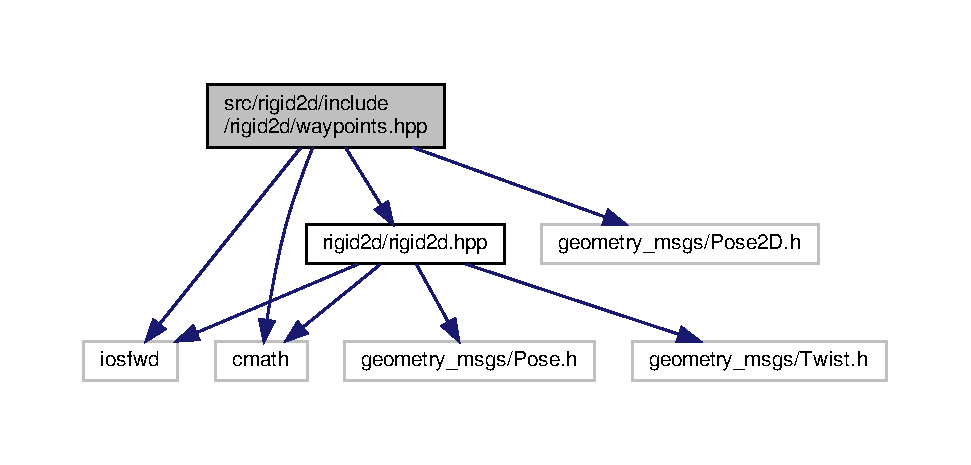
\includegraphics[width=350pt]{waypoints_8hpp__incl}
\end{center}
\end{figure}
\subsection*{Classes}
\begin{DoxyCompactItemize}
\item 
class \hyperlink{classrigid2d_1_1WayPoints}{rigid2d\+::\+Way\+Points}
\begin{DoxyCompactList}\small\item\em implements methods for navigating to a series of waypoints via a rotate and then translate strategy. \end{DoxyCompactList}\end{DoxyCompactItemize}


\subsection{Detailed Description}
Implements methods for navigating to a series of waypoints. 


%--- End generated contents ---

% Index
\backmatter
\newpage
\phantomsection
\clearemptydoublepage
\addcontentsline{toc}{chapter}{Index}
\printindex

\end{document}
